\documentclass[aspectratio=169, xcolor=dvipsnames]{beamer}

\usepackage{babel}
\usepackage{hyperref}
\usepackage{graphicx}
\usepackage{float}


\title{Advanced Topics in Databases}
\subtitle{Practical Assignment}

\author{Aníbal Silva \and Rui Fernandes}

\date{\today}

\begin{document}

\renewcommand{\today}{\ifcase \month\or January\or February\or March\or %
April\or May\or June\or July\or August\or September\or October\or November\or %
December\fi, \number \year}

\begin{frame}
    \titlepage
\end{frame}

\begin{frame}{Database}

\begin{block}{Some changed parameters:}

\begin{itemize}
    \item \texttt{athleteid} = \texttt{firstname} + \texttt{lastname} + \texttt{birthdate} + \texttt{inc\_id};
    \item \texttt{clubid} = \texttt{code} + \texttt{nation} + \texttt{region};
    \item \texttt{resultid} = \texttt{meetid} + \texttt{resultid};
    \item \texttt{swimstyleid} = \texttt{distance} + \texttt{relaycount} + \texttt{stroke};
    \item \texttt{eventid} = \texttt{meetid} + \texttt{eventid};
    \item The \texttt{license} = \texttt{athleteid} + \texttt{meetid}.
\end{itemize}
    
\end{block}

\begin{block}{PKs in fact tables:}
    \begin{itemize}
        \item \textit{Clubs de factos}, \texttt{pk\_clubfact} = \texttt{clubid} + \texttt{meetid} + \texttt{swimstyleid};
        \item \textit{Athlete de factos}, \texttt{pk\_athletefact} = \texttt{athleteid} + \texttt{from\_club} + \texttt{meetid}.
    \end{itemize}
\end{block}


\end{frame}

\begin{frame}{Database}
    \begin{figure}[H]
        \centering
        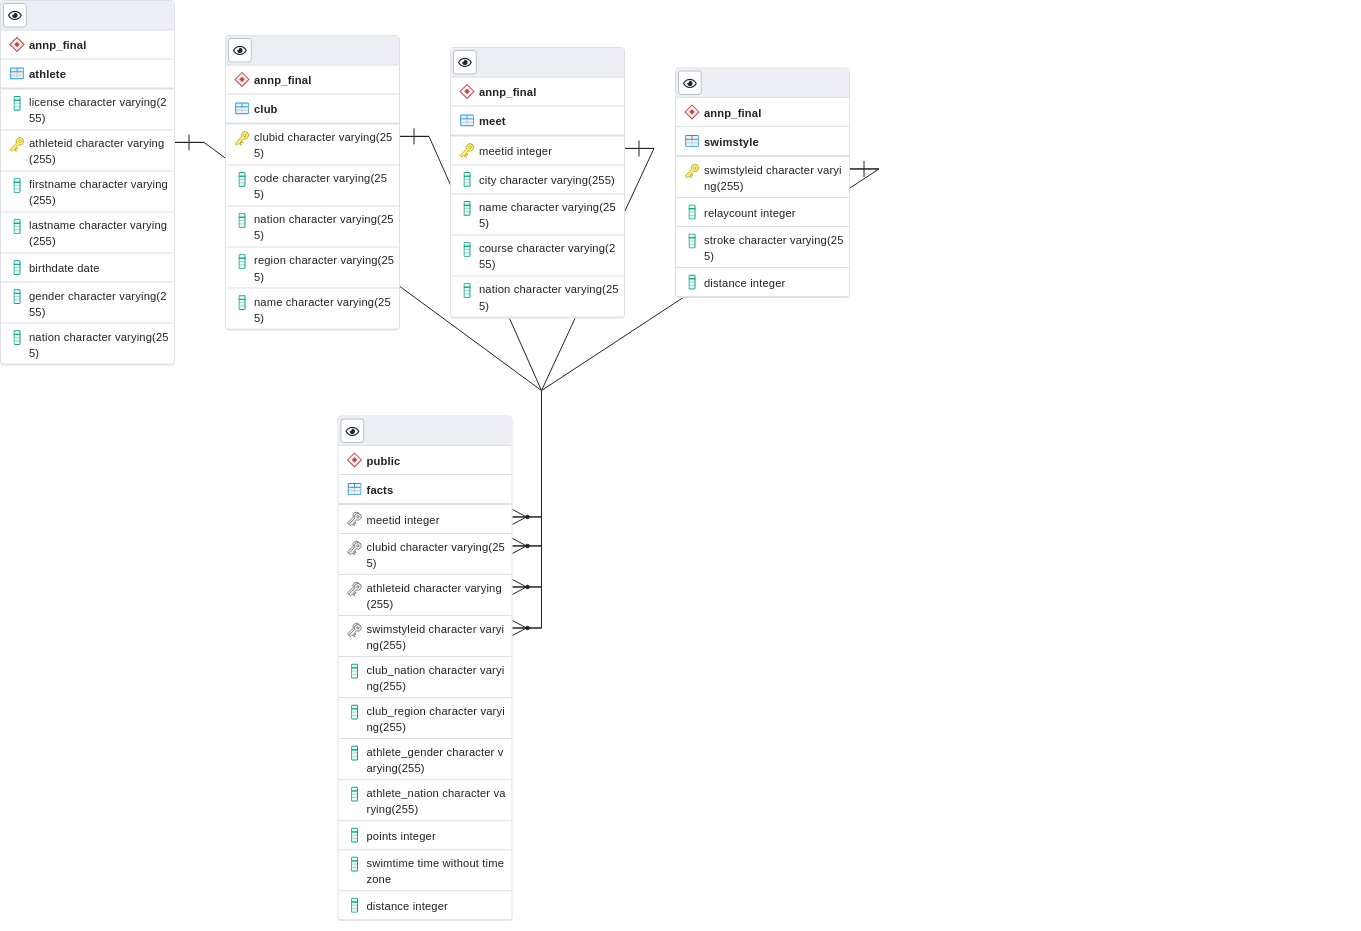
\includegraphics[width=.7\textwidth]{img/er.png}
    \end{figure}
\end{frame}

\begin{frame}{Average Age}
\begin{columns}[c]
% create the column with the first image, that  occupies
% half of the slide
\begin{column}{.5\textwidth}
\begin{figure}
    \centering
    
\includegraphics[width=0.9\textwidth]{img/sql/avgage.png}
\end{figure}
\end{column}

% create the column with the second image, that also
% occupies half of the slide
\begin{column}{.5\textwidth}
\begin{figure}
    \begin{itemize}
        \item \textbf{Average Age:} 46 years, 6 months and 31 days.
    \end{itemize}
\end{figure}
\end{column}
\end{columns}
\end{frame}

\begin{frame}{Youngest Athlete}
\begin{columns}[c]
% create the column with the first image, that  occupies
% half of the slide
\begin{column}{.5\textwidth}
\begin{figure}
    \centering
    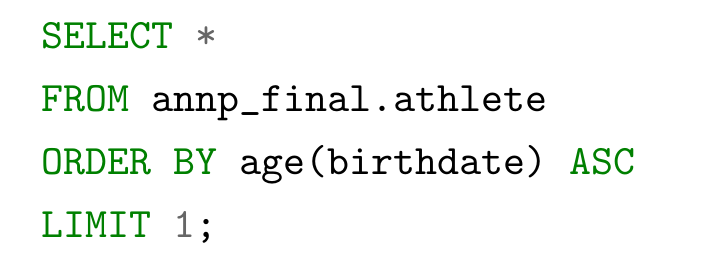
\includegraphics[width=0.9\textwidth]{img/sql/youngest.png}
\end{figure}
\end{column}

% create the column with the second image, that also
% occupies half of the slide
\begin{column}{.5\textwidth}
\begin{figure}
\begin{itemize}
    \item \textbf{Name:} Ana Mónica Eloi
    \item \textbf{Gender:} Female
    \item \textbf{Birthdate:} 29/12/1996
    \item \textbf{Age:} 25 years
\end{itemize}
\end{figure}
\end{column}
\end{columns}
\end{frame}

\begin{frame}{Oldest Athlete}
\begin{columns}[c]
% create the column with the first image, that  occupies
% half of the slide
\begin{column}{.5\textwidth}
\begin{figure}
    \centering
    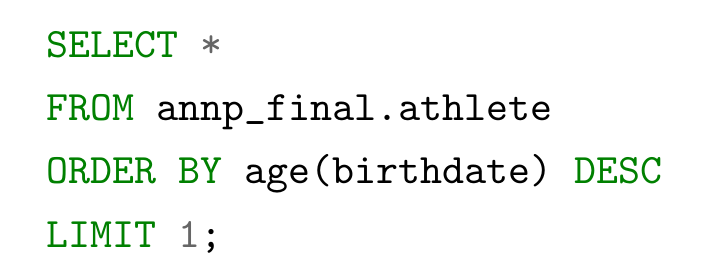
\includegraphics[width=0.9\textwidth]{img/sql/oldest.png}
\end{figure}
\end{column}

% create the column with the second image, that also
% occupies half of the slide
\begin{column}{.5\textwidth}
\begin{figure}
\begin{itemize}
    \item \textbf{Name:} Virgílio Zacarias Costa
    \item \textbf{Gender:} Male
    \item \textbf{Birthdate:} 21/07/1931
    \item \textbf{Age:} 90 years
\end{itemize}
\end{figure}
\end{column}
\end{columns}
\end{frame}

\begin{frame}{Athletes by Age}
\begin{columns}[c]
% create the column with the first image, that  occupies
% half of the slide
\begin{column}{.5\textwidth}
\begin{figure}
    \centering
    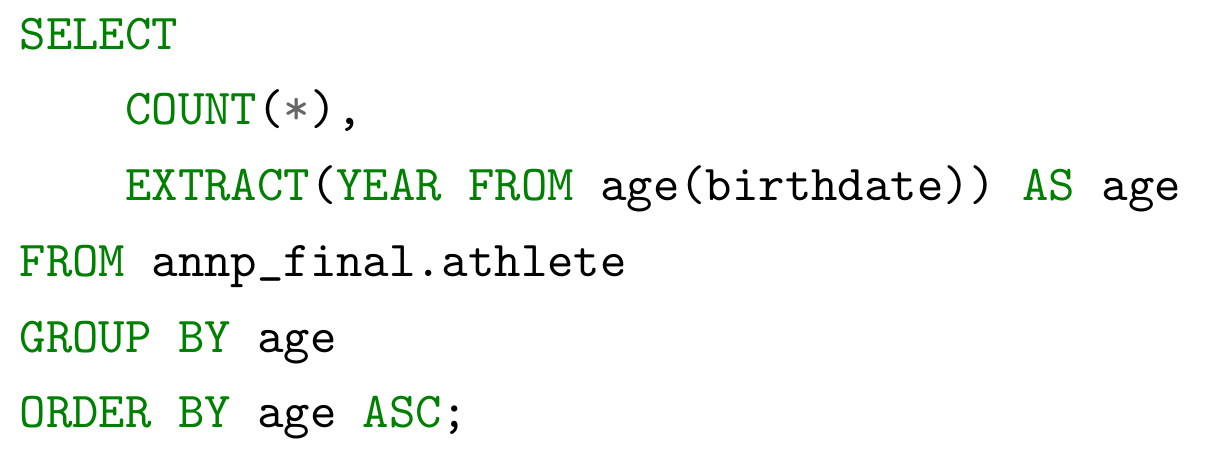
\includegraphics[width=\textwidth]{img/sql/athletesbyage.png}
\end{figure}
\end{column}

% create the column with the second image, that also
% occupies half of the slide
\begin{column}{.5\textwidth}
\begin{figure}
    \centering
    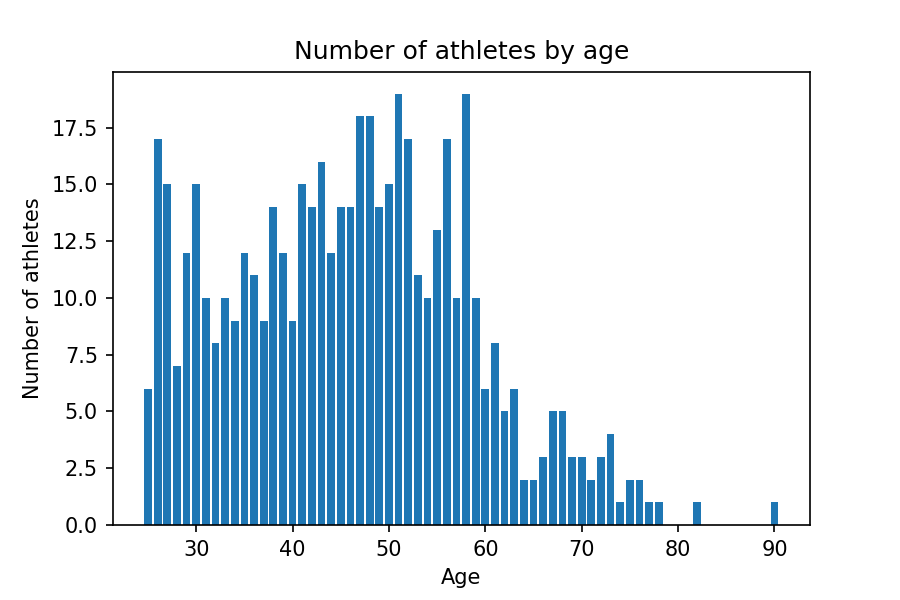
\includegraphics[width=\textwidth]{img/athletesbyage.png}
\end{figure}
\end{column}
\end{columns}
\end{frame}

\begin{frame}{Athletes by Age \& Gender}
\begin{columns}[c]
% create the column with the first image, that  occupies
% half of the slide
\begin{column}{.5\textwidth}
\begin{figure}
    \centering
    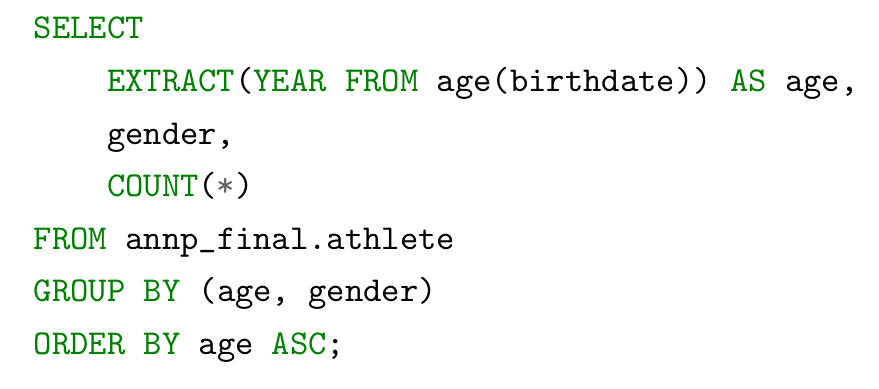
\includegraphics[width=\textwidth]{img/sql/ageandgender.png}
\end{figure}
\end{column}

% create the column with the second image, that also
% occupies half of the slide
\begin{column}{.5\textwidth}
\begin{figure}
    \centering
    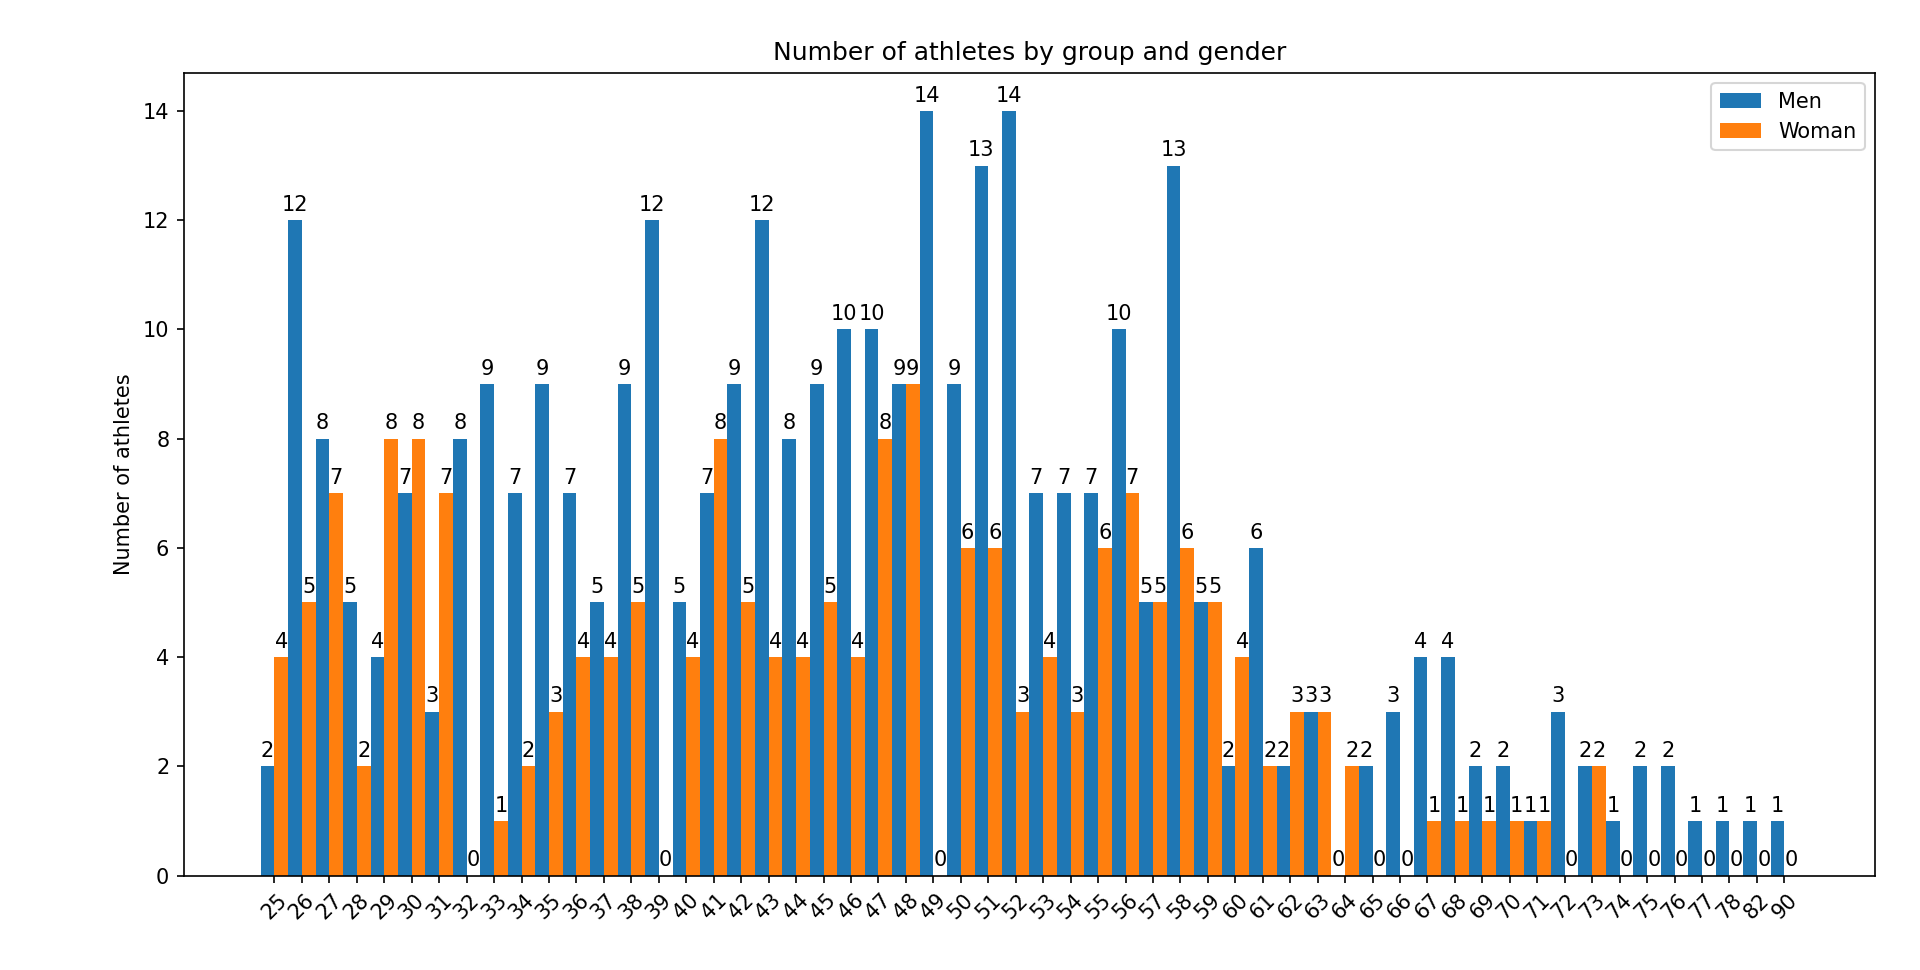
\includegraphics[width=\textwidth]{img/athletesbyageandgender.png}
\end{figure}
\end{column}
\end{columns}
\end{frame}

\begin{frame}
\begin{figure}
    \centering
    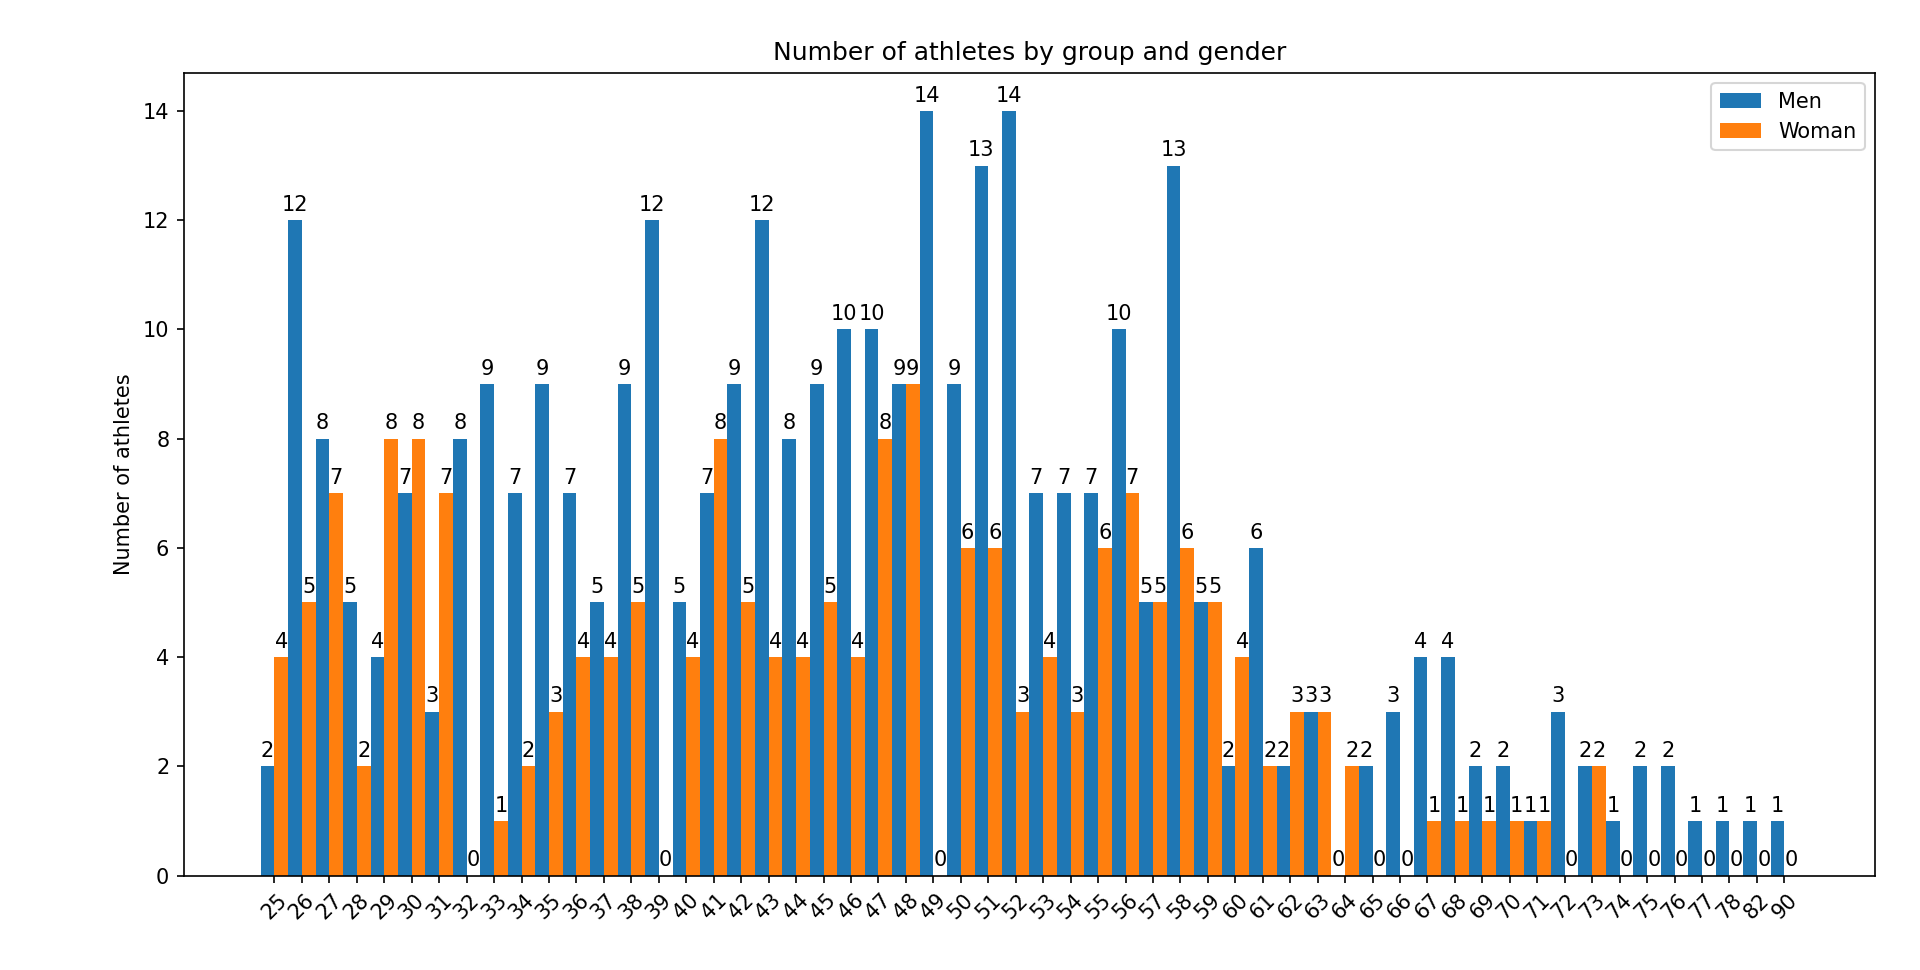
\includegraphics[width=\textwidth]{img/athletesbyageandgender.png}
\end{figure}
\end{frame}

\begin{frame}{Athletes by Nation}
\begin{columns}[c]
% create the column with the first image, that  occupies
% half of the slide
\begin{column}{.4\textwidth}
\begin{figure}
    \centering
    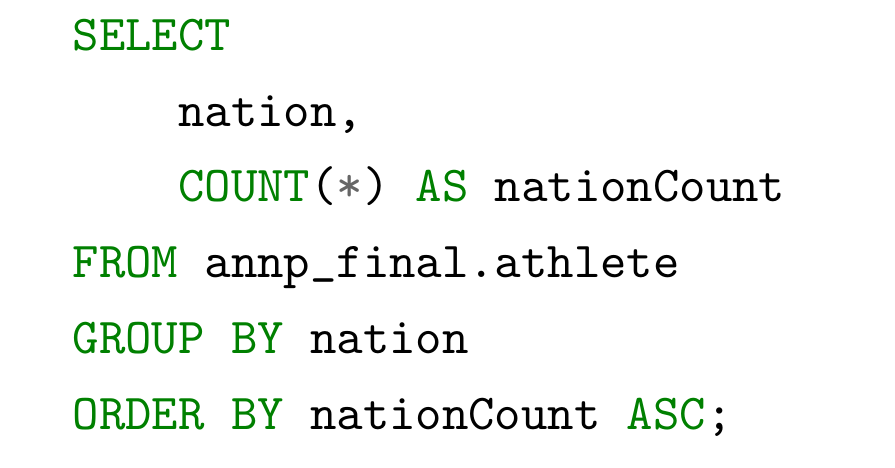
\includegraphics[width=\textwidth]{img/sql/nation.png}
\end{figure}
\end{column}

% create the column with the second image, that also
% occupies half of the slide
\begin{column}{.6\textwidth}
\begin{figure}
    \centering
    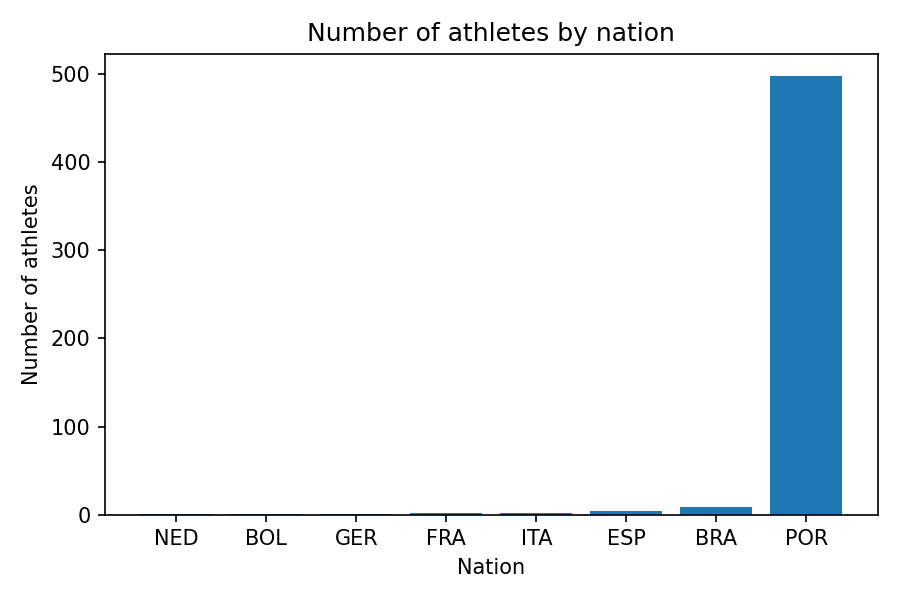
\includegraphics[width=\textwidth]{img/athletesbynation.png}
\end{figure}
\end{column}
\end{columns}
\end{frame}

\begin{frame}{Athletes by Nation \& Gender}
\begin{columns}[c]
% create the column with the first image, that  occupies
% half of the slide
\begin{column}{.5\textwidth}
\begin{figure}
    \centering
    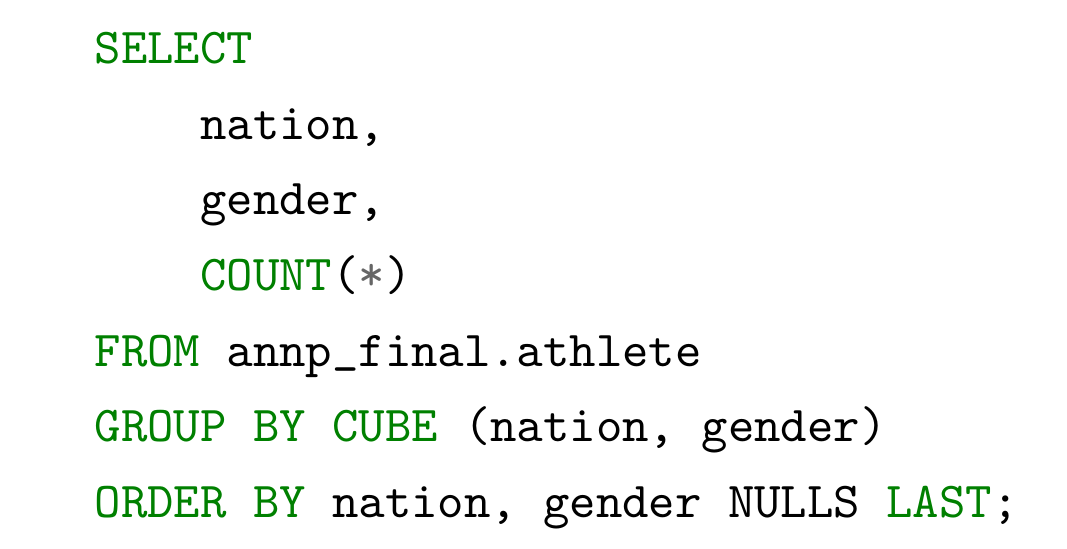
\includegraphics[width=\textwidth]{img/sql/nationgender.png}
\end{figure}
\end{column}

% create the column with the second image, that also
% occupies half of the slide
\begin{column}{.5\textwidth}
\begin{figure}
    \centering
    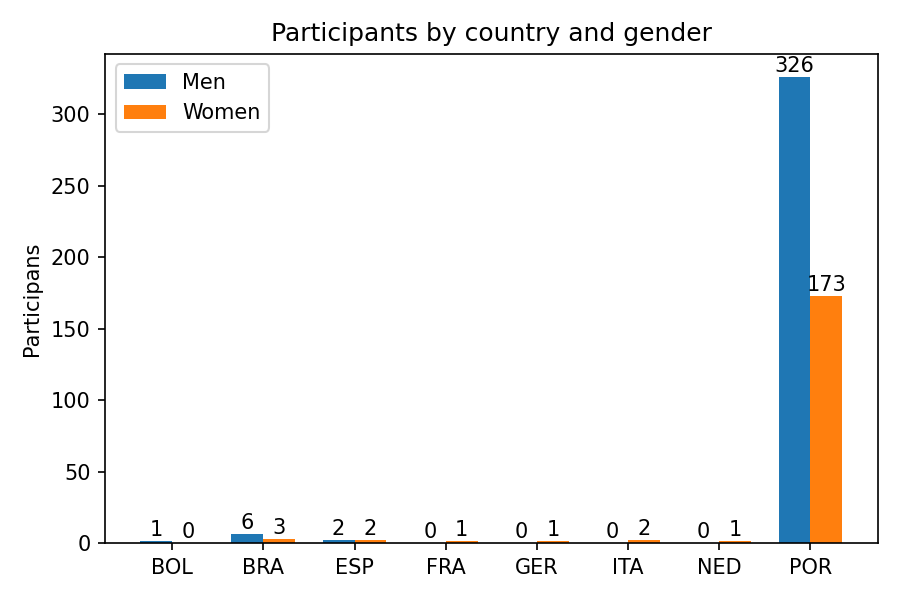
\includegraphics[width=\textwidth]{img/athletesbynationgender.png}
\end{figure}
\end{column}
\end{columns}
\end{frame}

\begin{frame}{Athletes by Gender}
\begin{columns}[c]
% create the column with the first image, that  occupies
% half of the slide
\begin{column}{.5\textwidth}
\begin{figure}
    \centering
    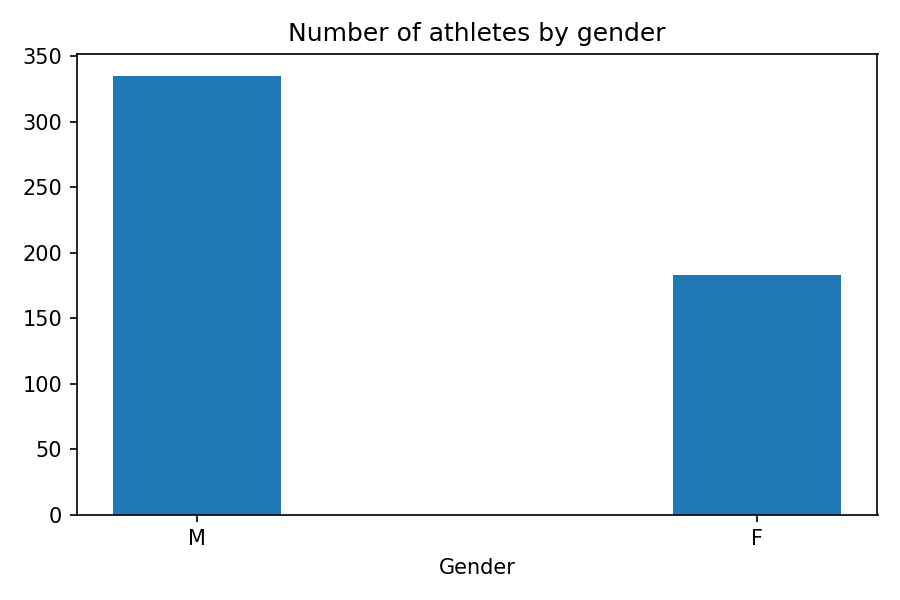
\includegraphics[width=\textwidth]{img/athletesbygender.png}
\end{figure}
\end{column}

% create the column with the second image, that also
% occupies half of the slide
\begin{column}{.5\textwidth}
\begin{figure}
    \centering
    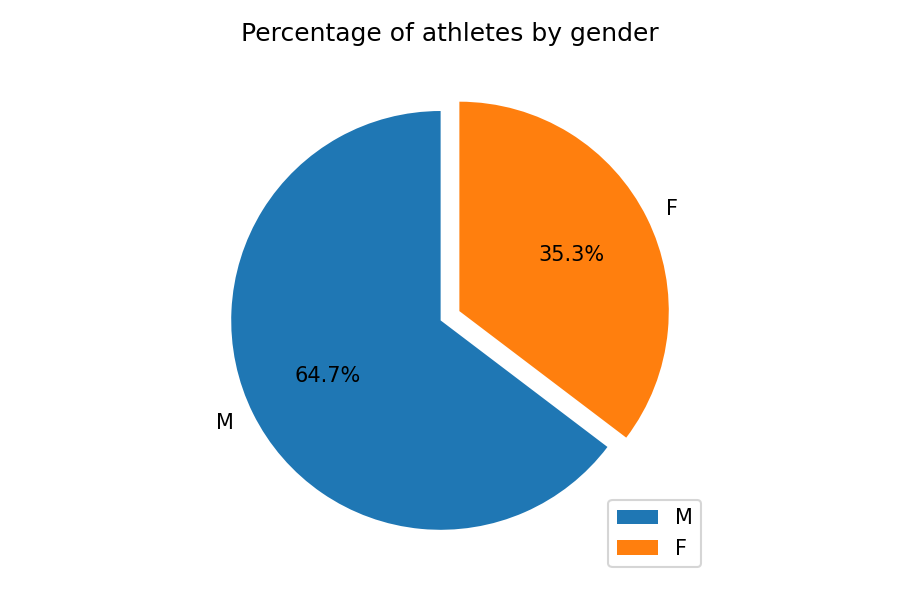
\includegraphics[width=\textwidth]{img/athletesbygender-pie.png}
\end{figure}
\end{column}
\end{columns}
\end{frame}

\begin{frame}{Clubs by Nation}
\begin{columns}[c]
% create the column with the first image, that  occupies
% half of the slide
\begin{column}{.45\textwidth}
\begin{figure}
    \centering
    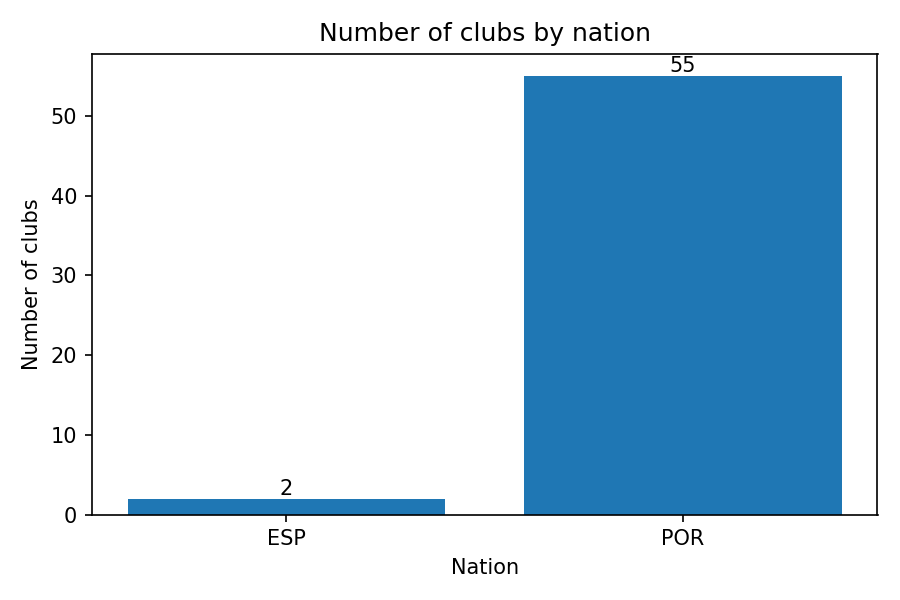
\includegraphics[width=\textwidth]{img/clubsbynation.png}
\end{figure}
\end{column}

% create the column with the second image, that also
% occupies half of the slide
\begin{column}{.55\textwidth}
\begin{figure}
    \centering
    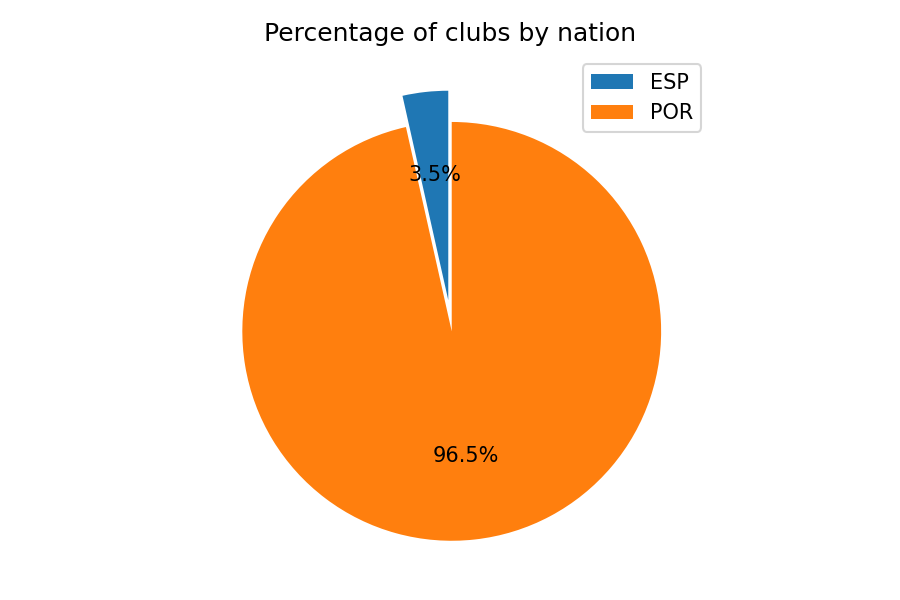
\includegraphics[width=\textwidth]{img/clubsbynation-pie.png}
\end{figure}
\end{column}
\end{columns}
\end{frame}

\begin{frame}{Clubs by Region (PT)}
\begin{columns}[c]
% create the column with the first image, that  occupies
% half of the slide
\begin{column}{.45\textwidth}
\begin{figure}
    \centering
    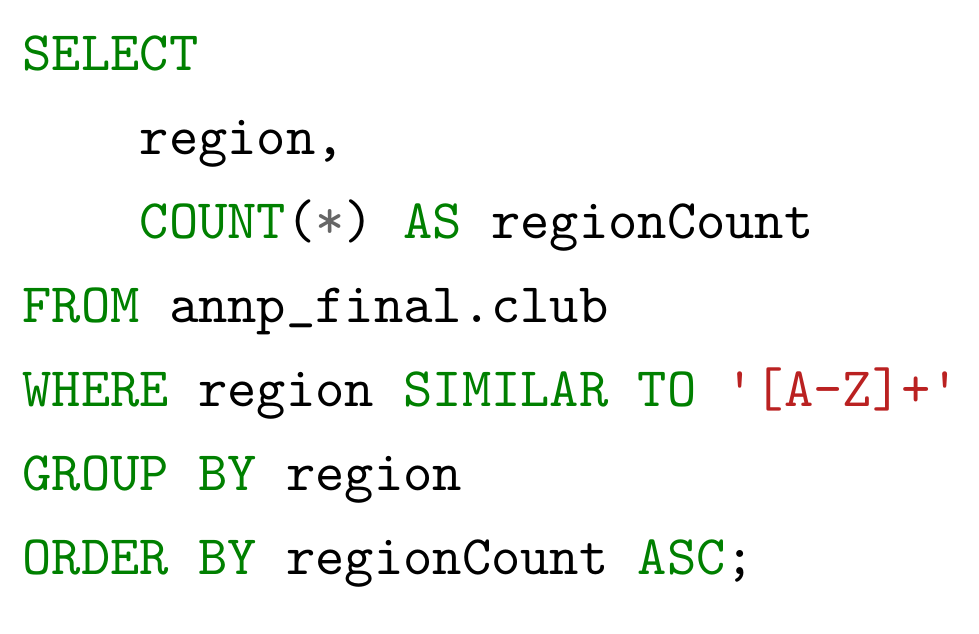
\includegraphics[width=\textwidth]{img/sql/clubsregionpt.png}
\end{figure}
\end{column}

% create the column with the second image, that also
% occupies half of the slide
\begin{column}{.55\textwidth}
\begin{figure}
    \centering
    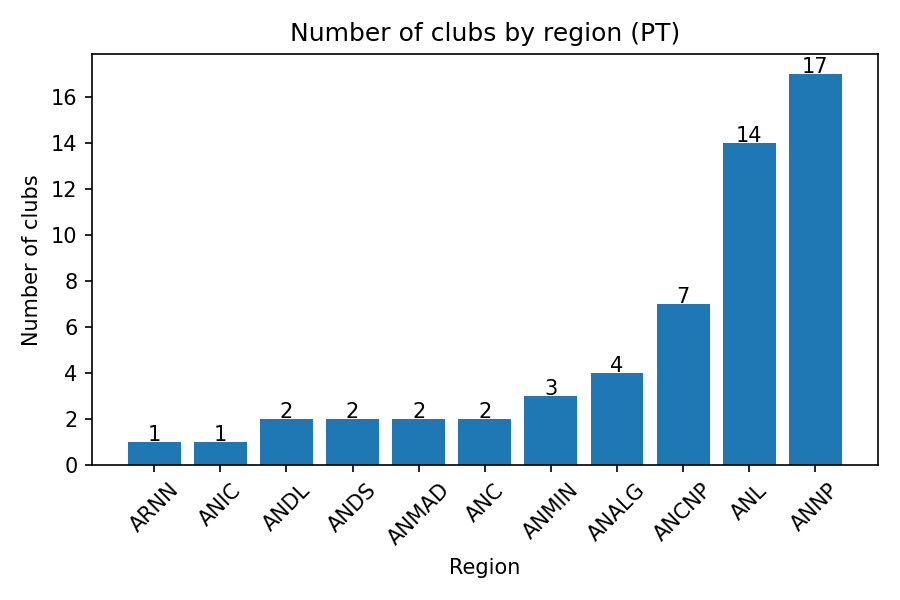
\includegraphics[width=\textwidth]{img/clubsbyregion-pt.png}
\end{figure}
\end{column}
\end{columns}
\end{frame}

\begin{frame}{Clubs by Region (ES)}
\begin{columns}[c]
% create the column with the first image, that  occupies
% half of the slide
\begin{column}{.45\textwidth}
\begin{figure}
    \centering
    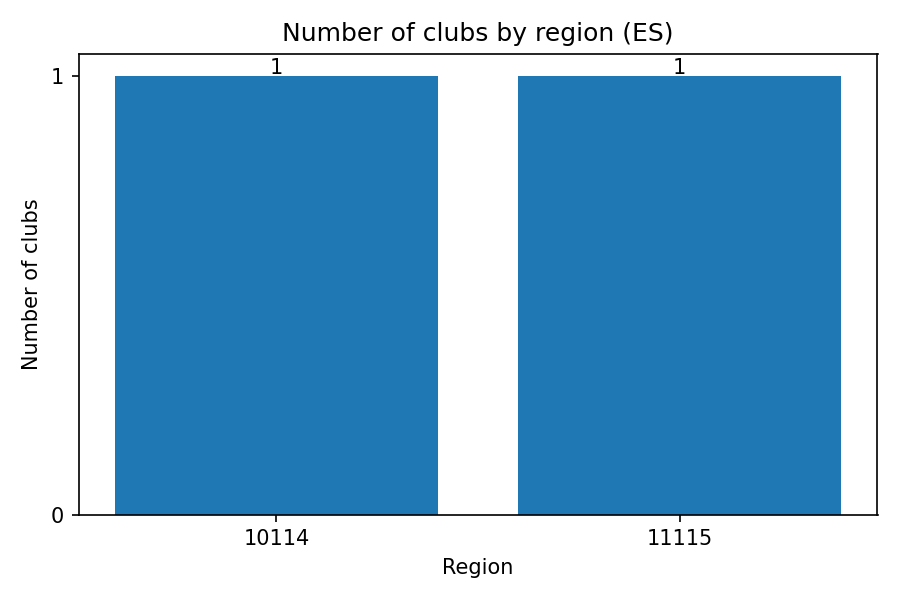
\includegraphics[width=\textwidth]{img/clubsbyregion-es.png}
\end{figure}
\end{column}

% create the column with the second image, that also
% occupies half of the slide
\begin{column}{.55\textwidth}
\begin{figure}
    \centering
    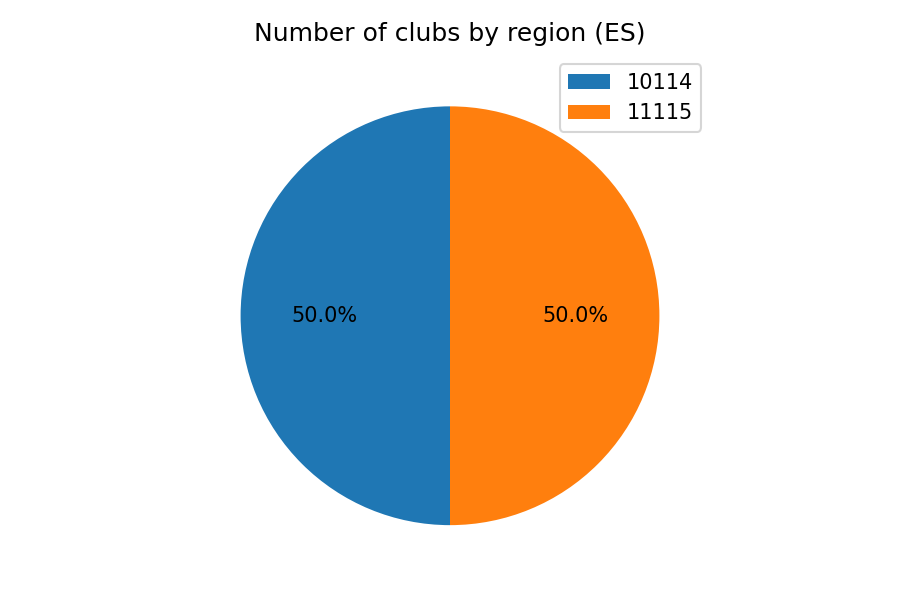
\includegraphics[width=\textwidth]{img/clubsbyregion-es-pie.png}
\end{figure}
\end{column}
\end{columns}

\end{frame}

\begin{frame}{Club Fact statistics}

\begin{figure}
    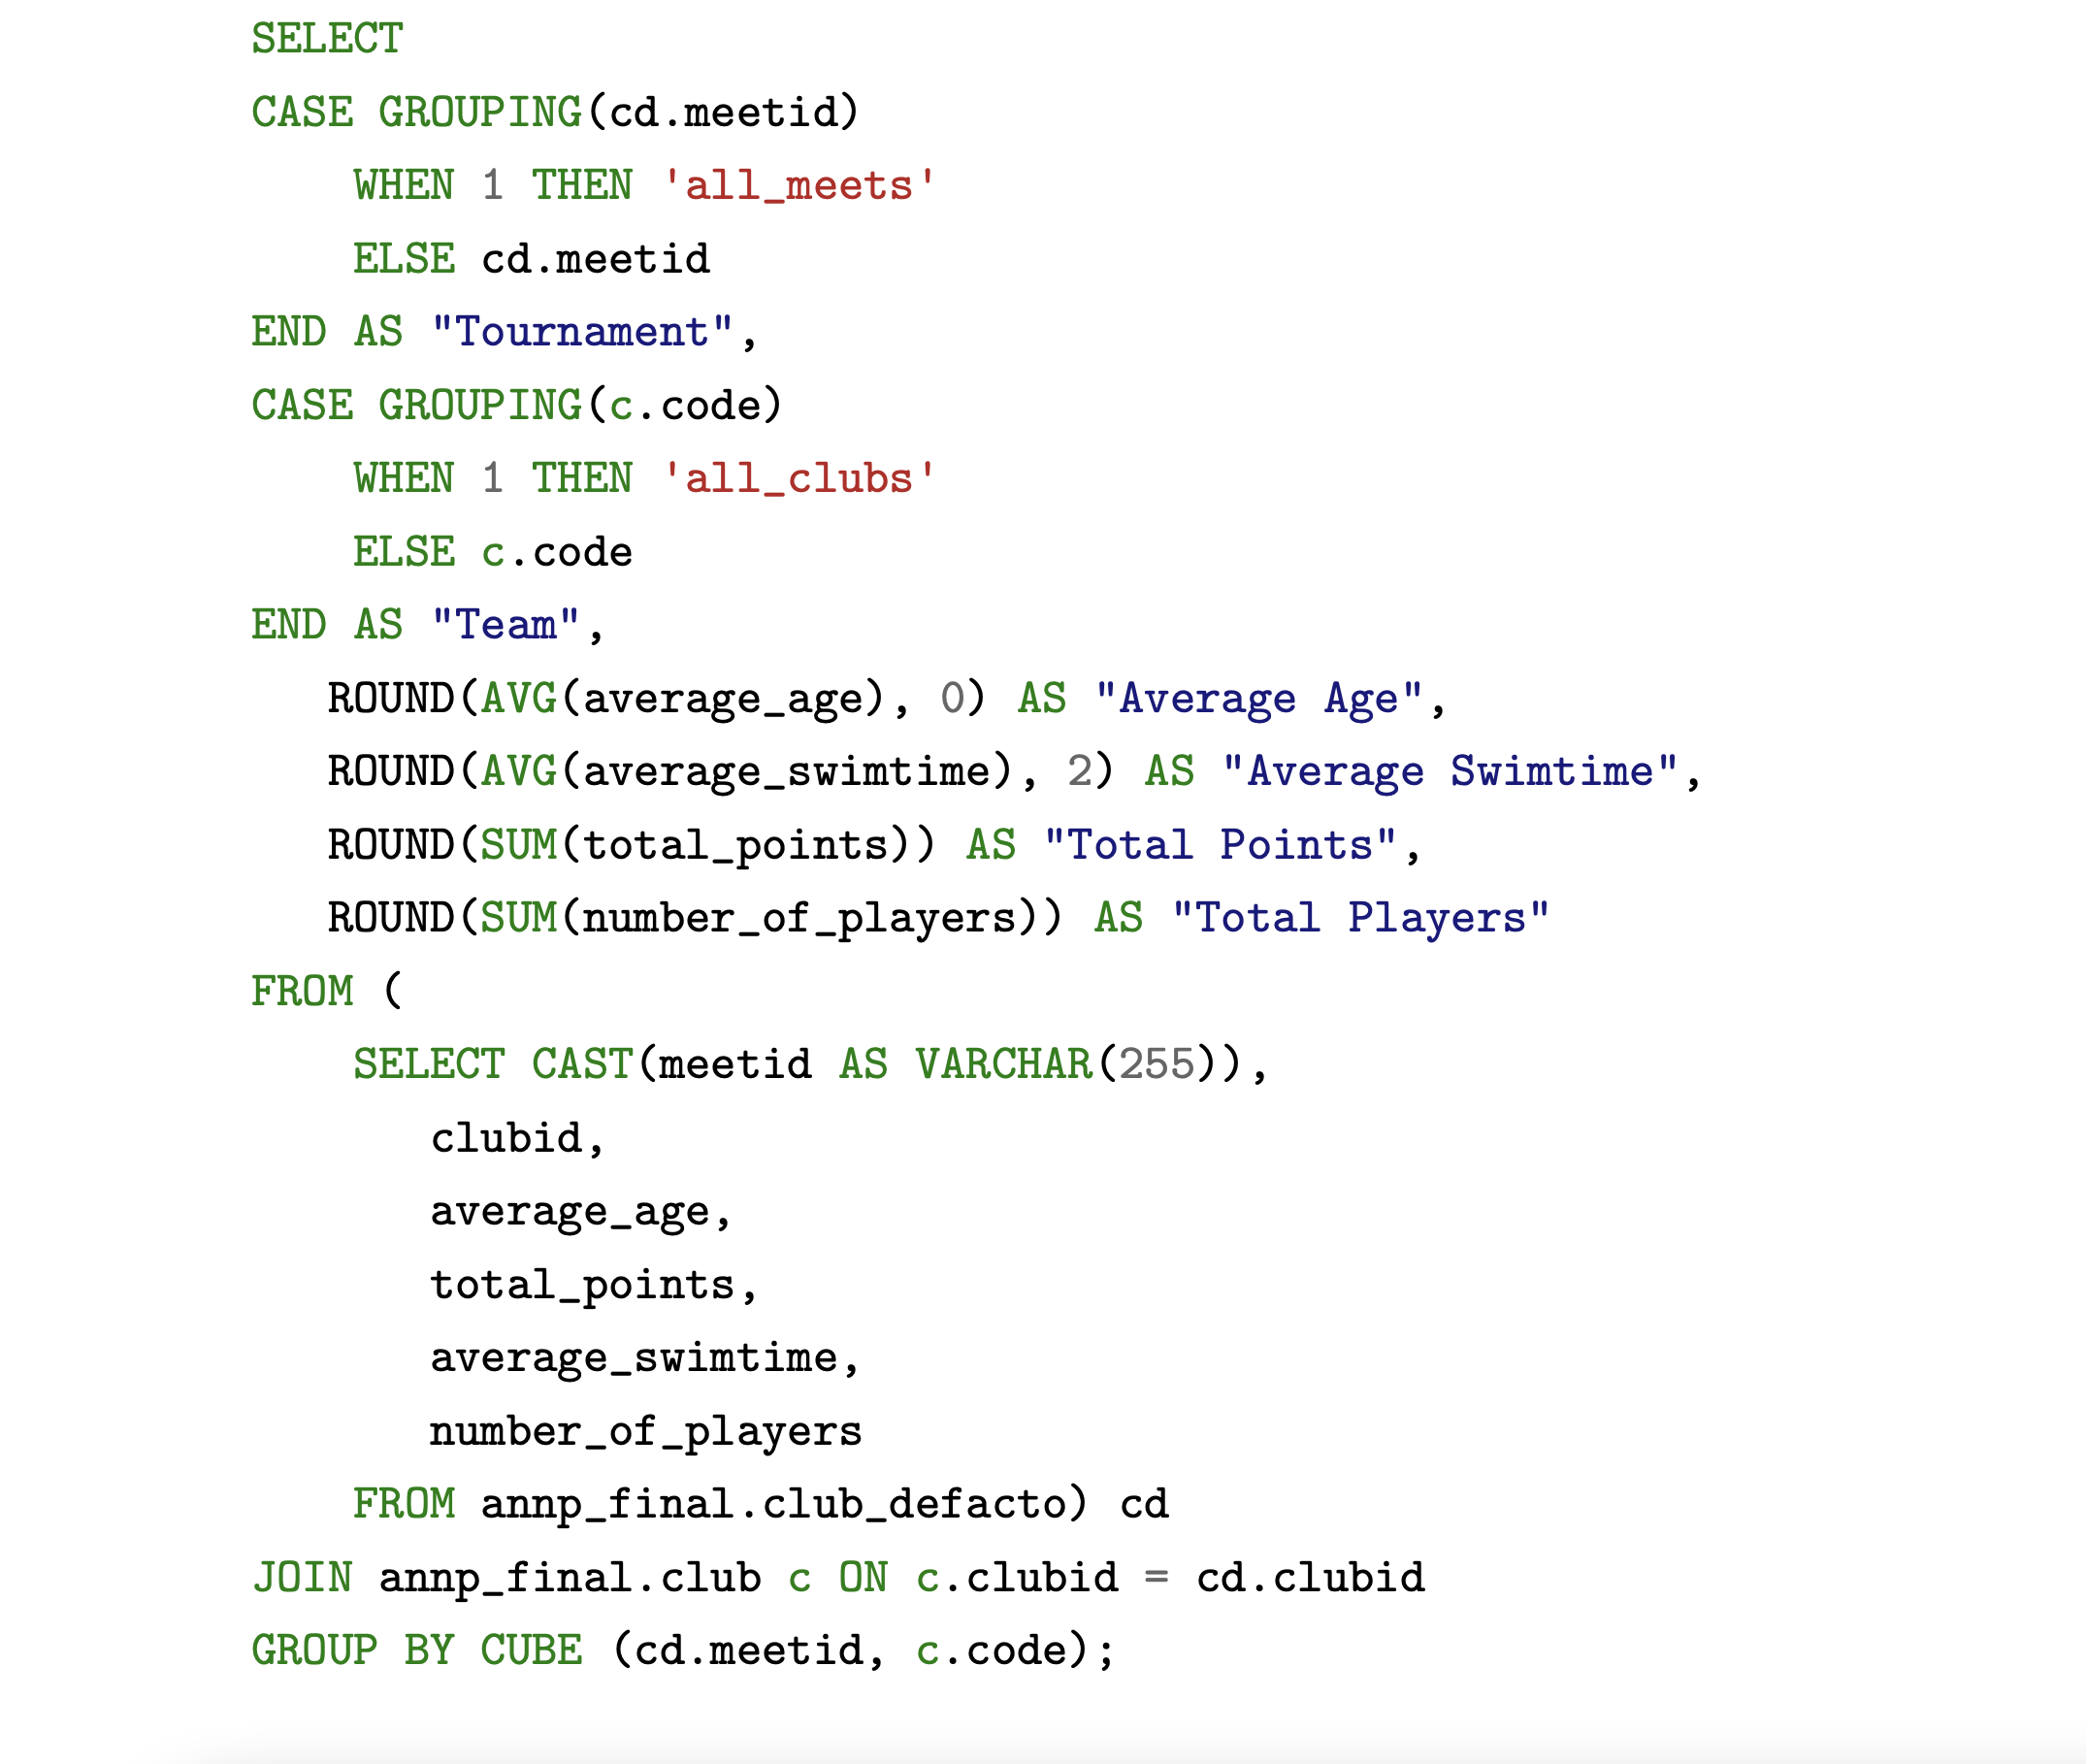
\includegraphics[scale=0.2]{img/clubs-stats-all.png}\hspace*{10cm}
\end{figure}

\end{frame}

\begin{frame}[allowframebreaks]{Overall Club Statistics}
\begin{figure}
    \centering
    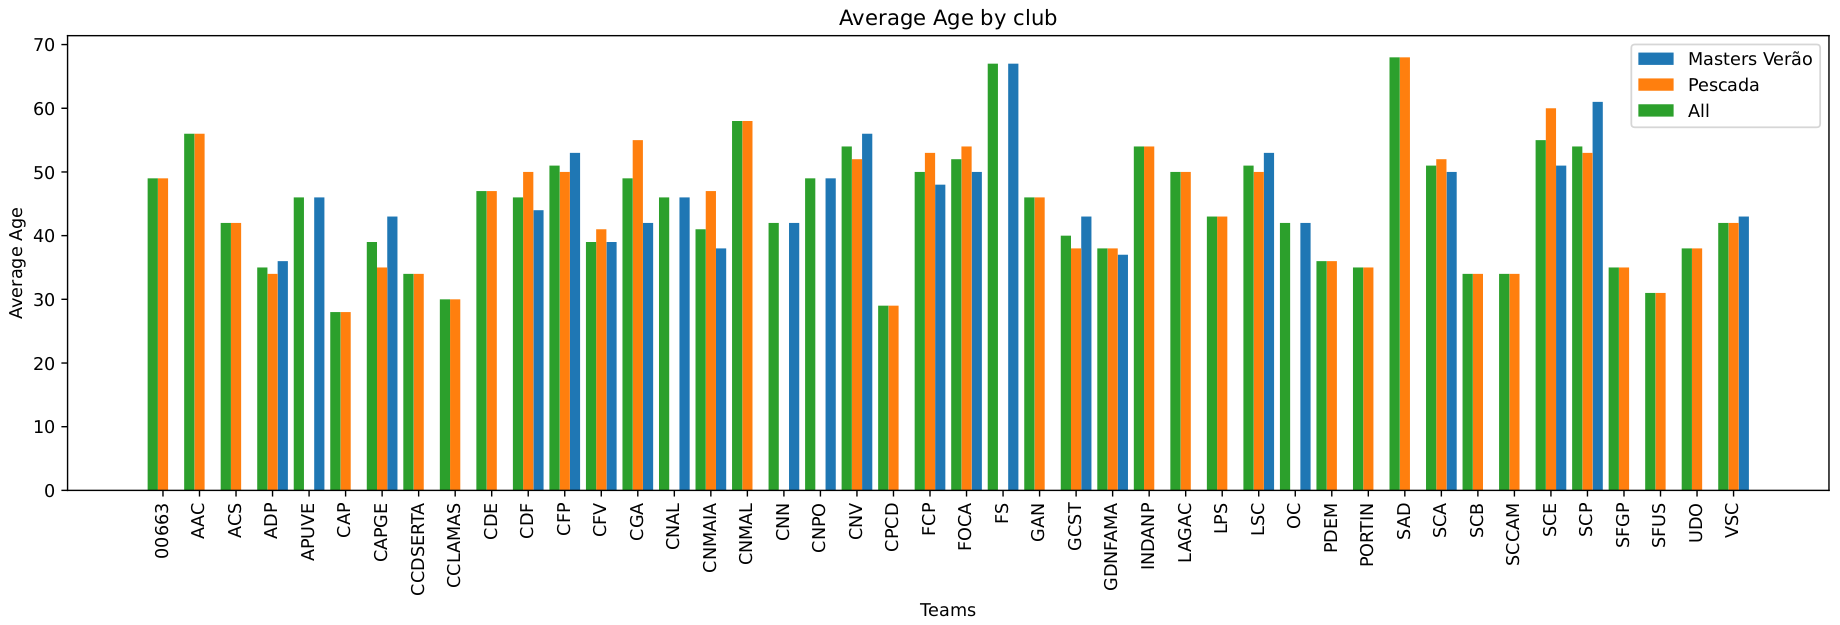
\includegraphics[width=\textwidth]{img/stats/clubfacts1.png}
\end{figure}

\begin{figure}
    \centering
    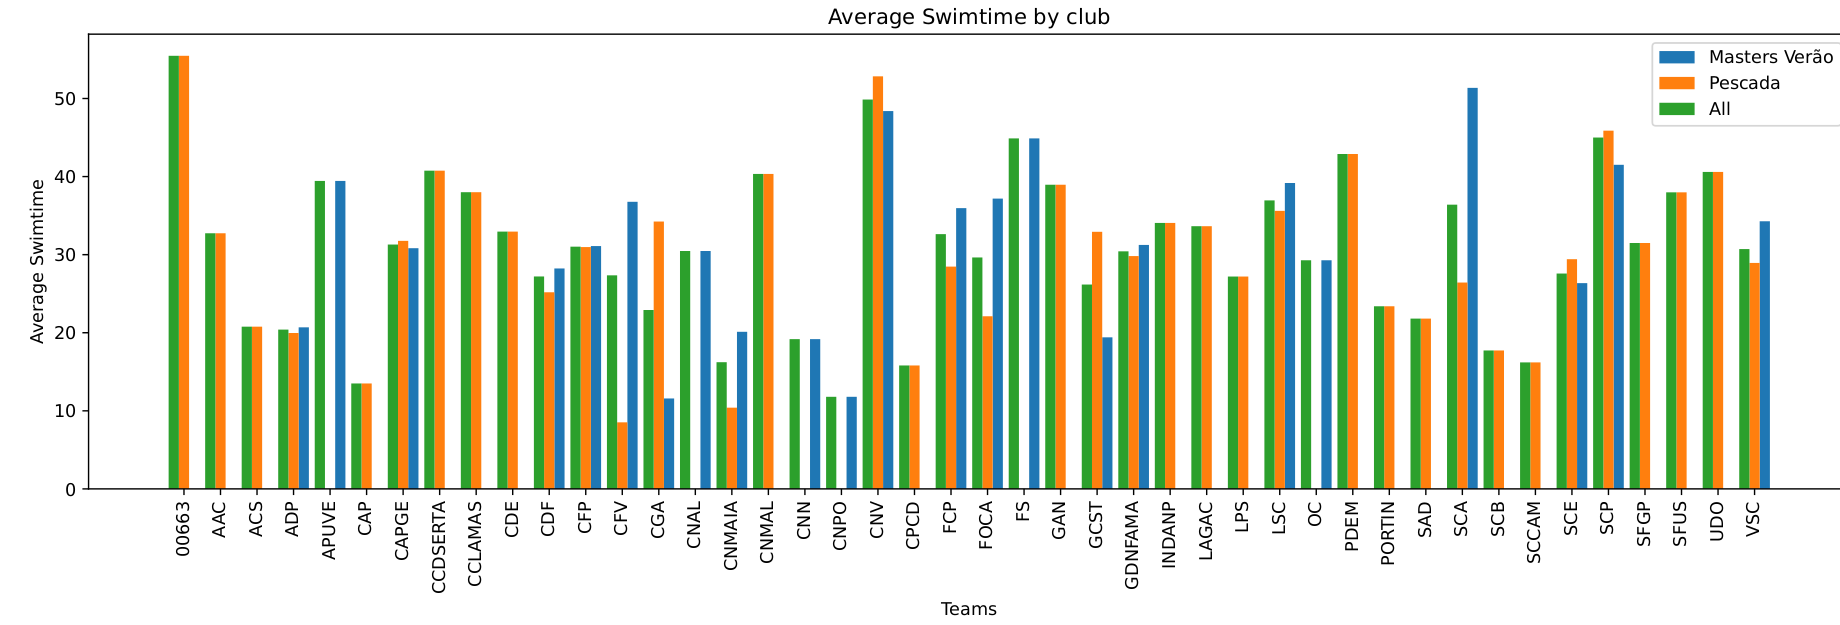
\includegraphics[width=\textwidth]{img/stats/clubfacts2.png}
\end{figure}

\begin{figure}
    \centering
    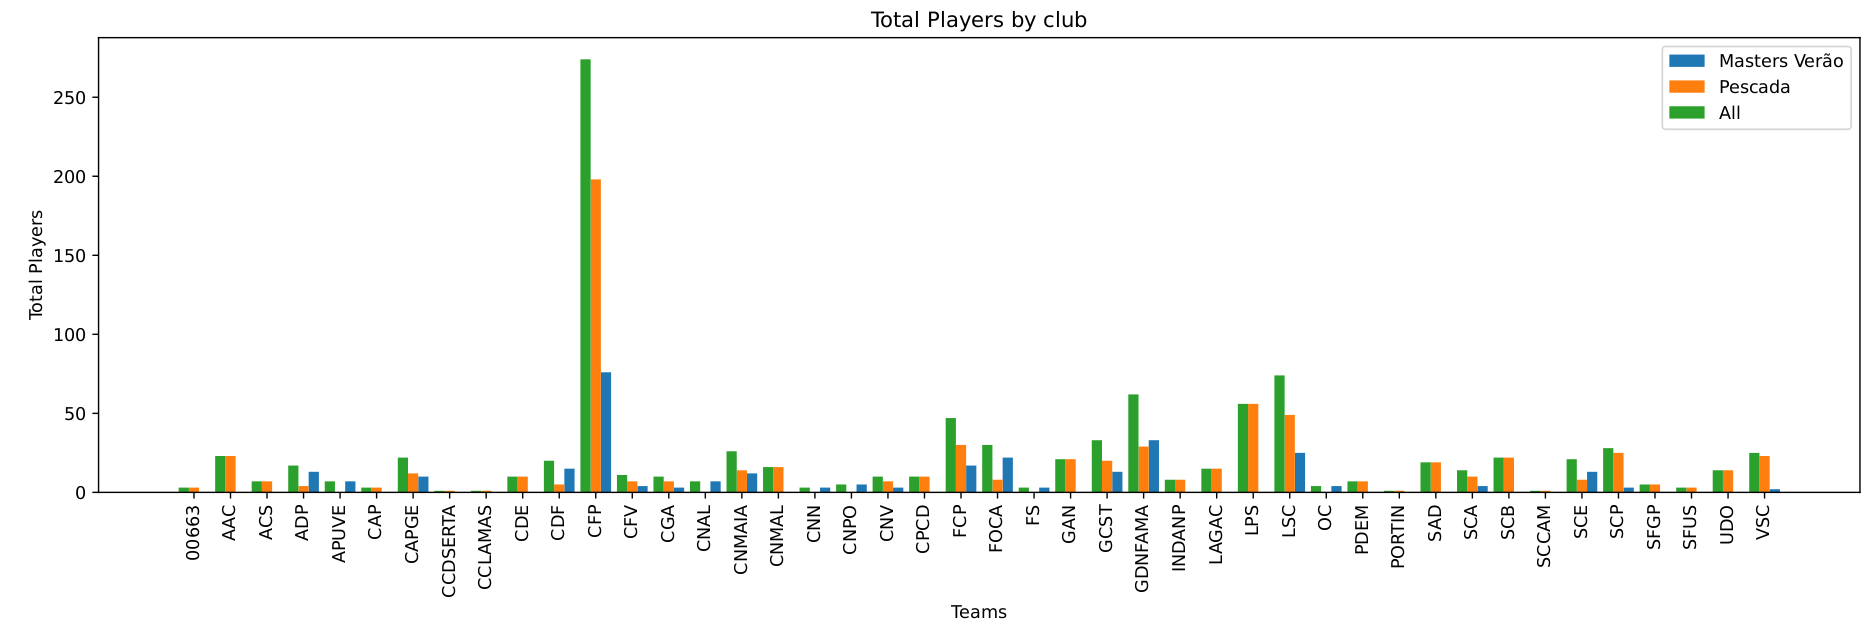
\includegraphics[width=\textwidth]{img/stats/clubfacts3.png}
\end{figure}

\begin{figure}
    \centering
    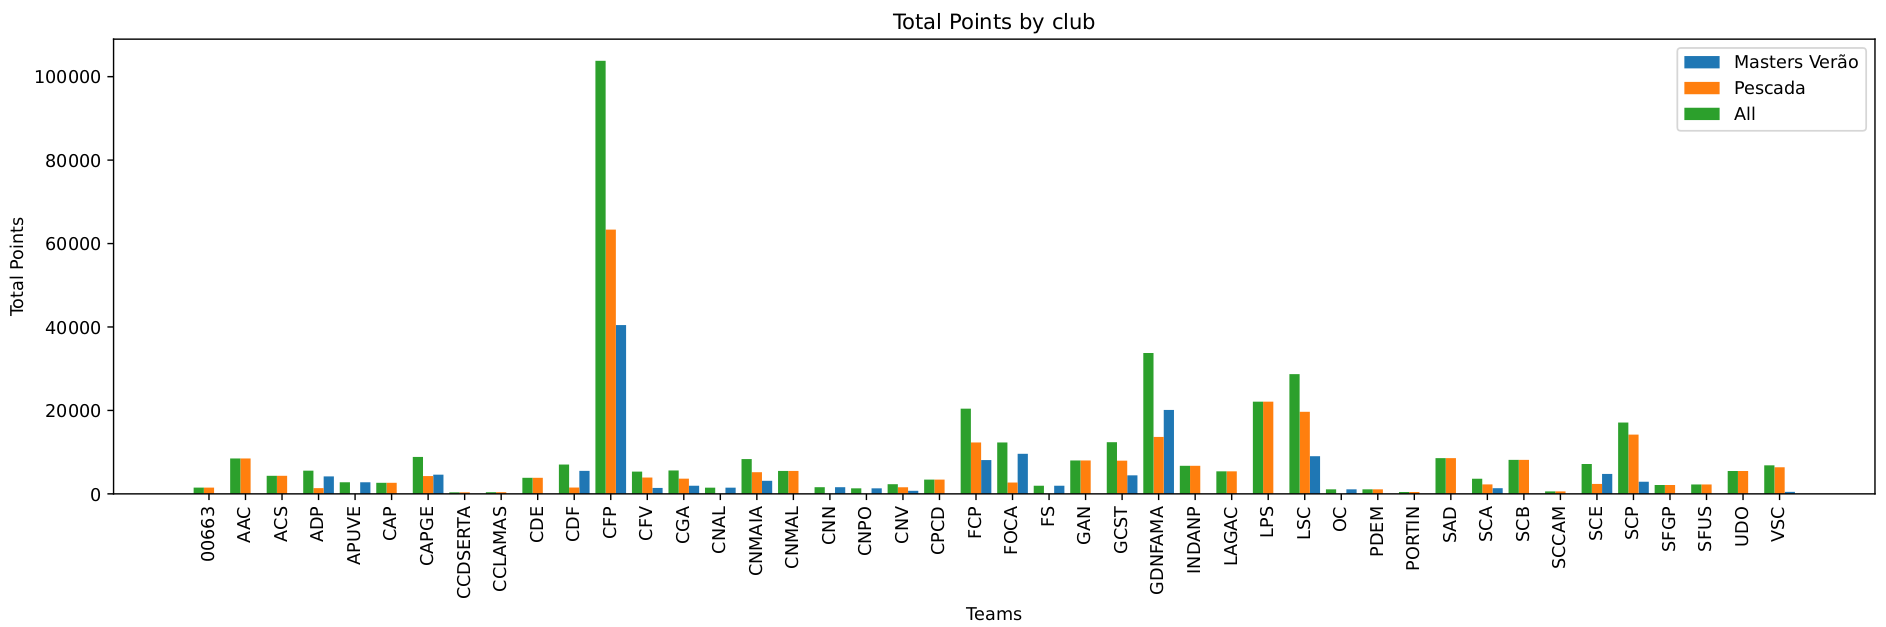
\includegraphics[width=\textwidth]{img/stats/clubfacts4.png}
\end{figure}

\end{frame}

\begin{frame}{Swim Style Statistics By Club}

\begin{figure}
    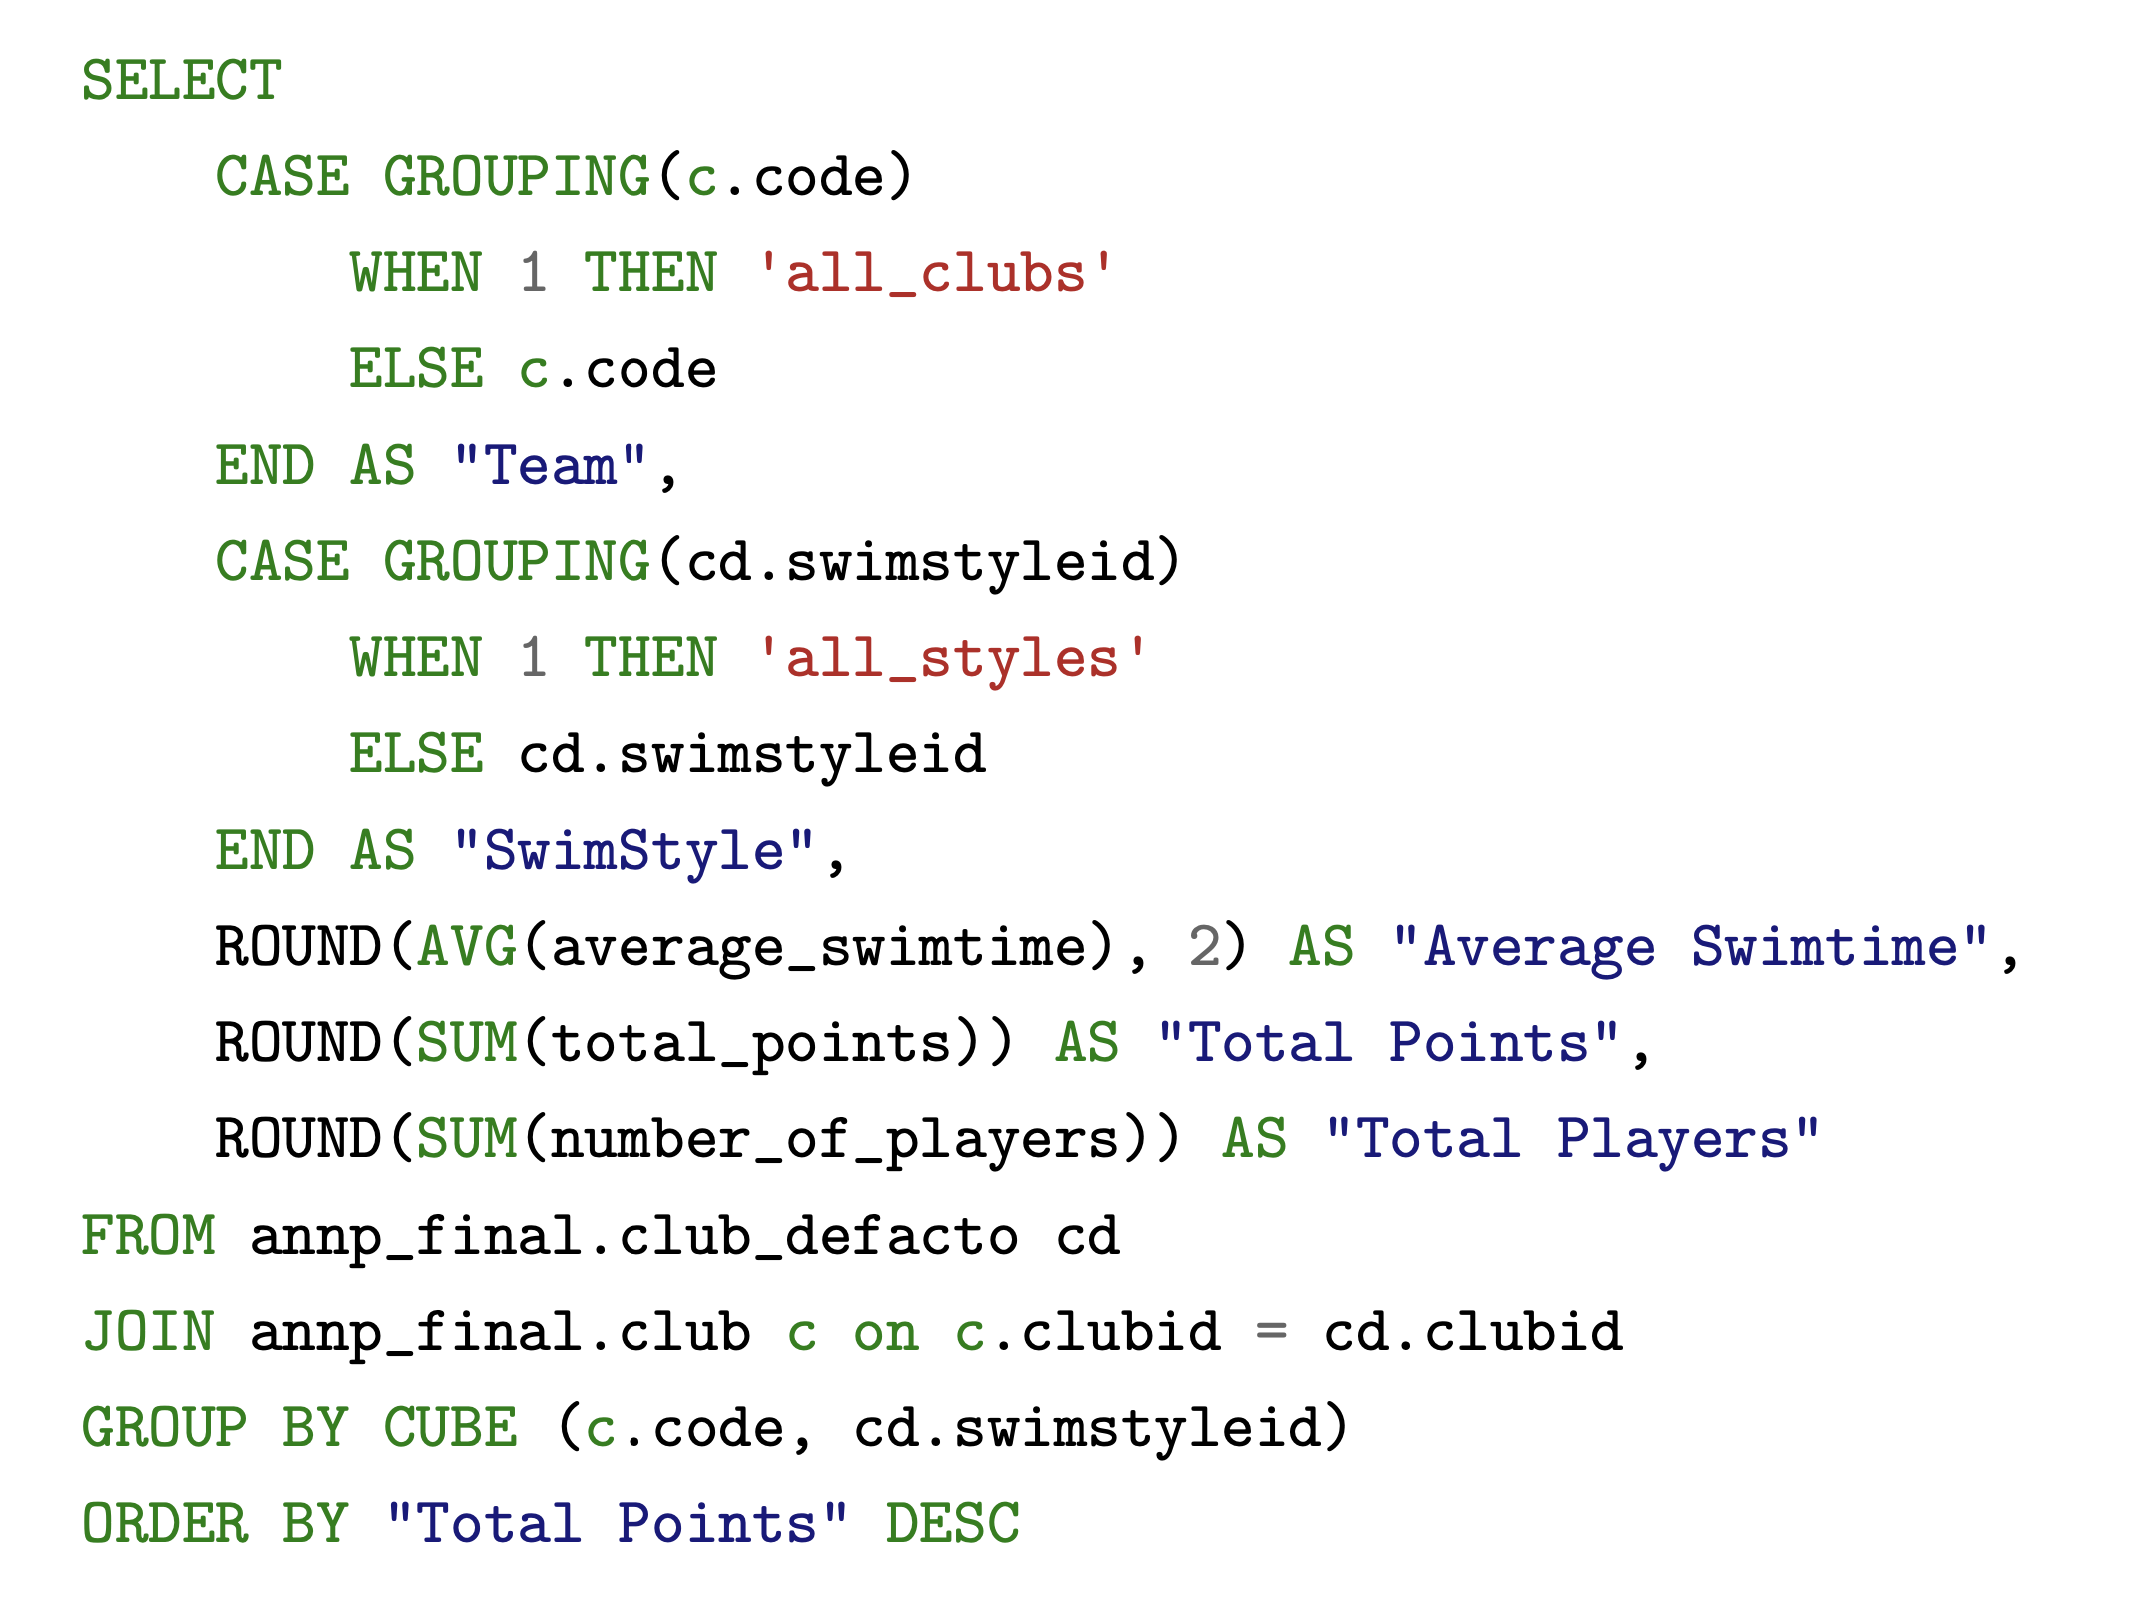
\includegraphics[scale=0.25]{img/clubs-stats-swim.png}\hspace*{10cm}
\end{figure}

\end{frame}

\begin{frame}{Swim Style Statistics}
\begin{figure}
    \centering
    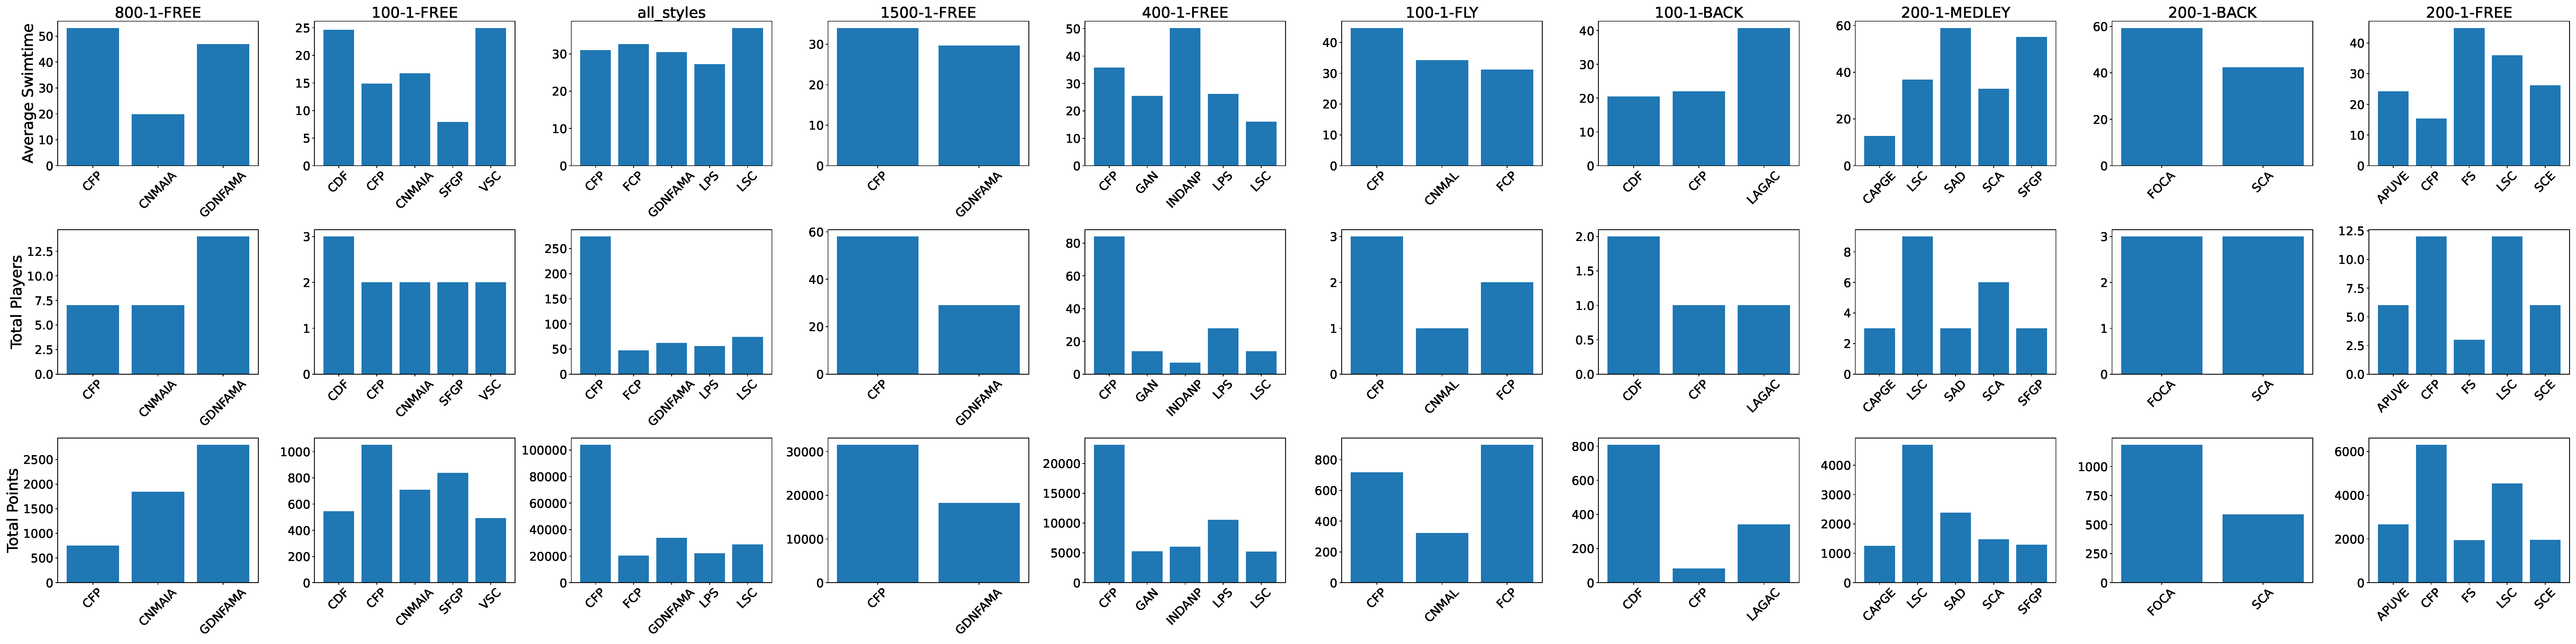
\includegraphics[width=\textwidth]{img/stats_clubs_swim.pdf}
\end{figure}
\end{frame}


\begin{frame}{Athlete Fact Statistics}
\begin{figure}
    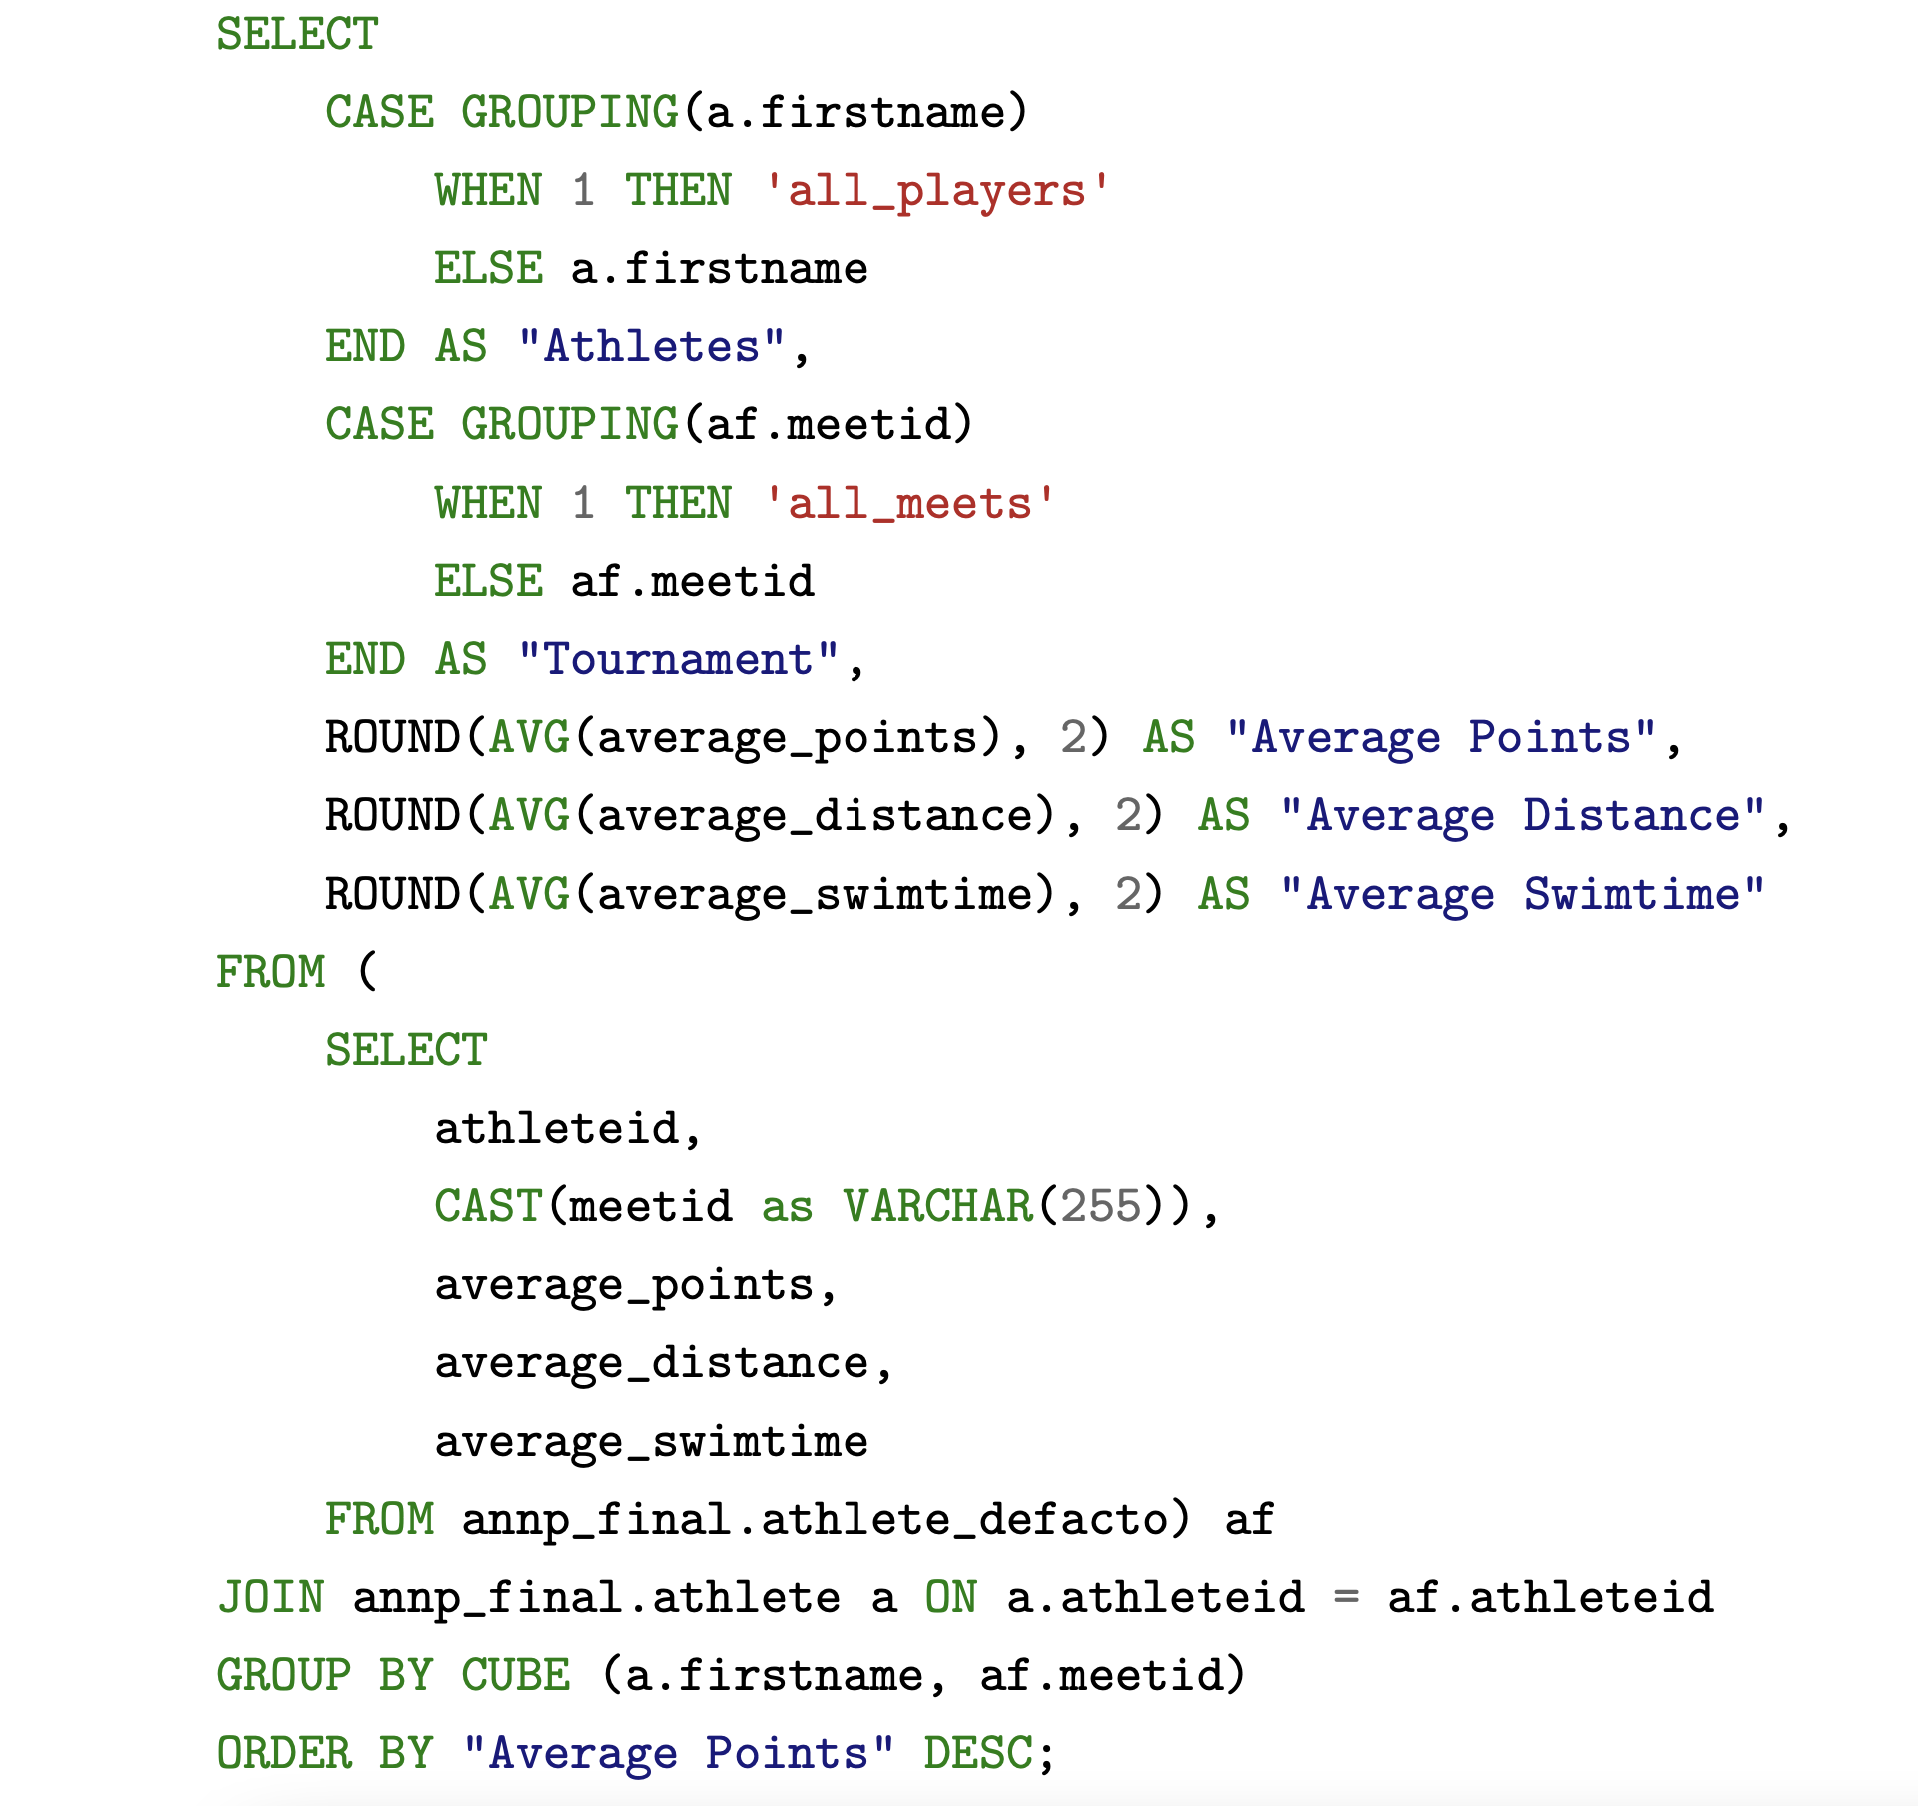
\includegraphics[scale=0.2]{img/athletes-stats.png}\hspace*{10cm}
\end{figure}
\end{frame}


\begin{frame}[allowframebreaks]{Overall Athlete Statistics}
\begin{figure}
    \centering
    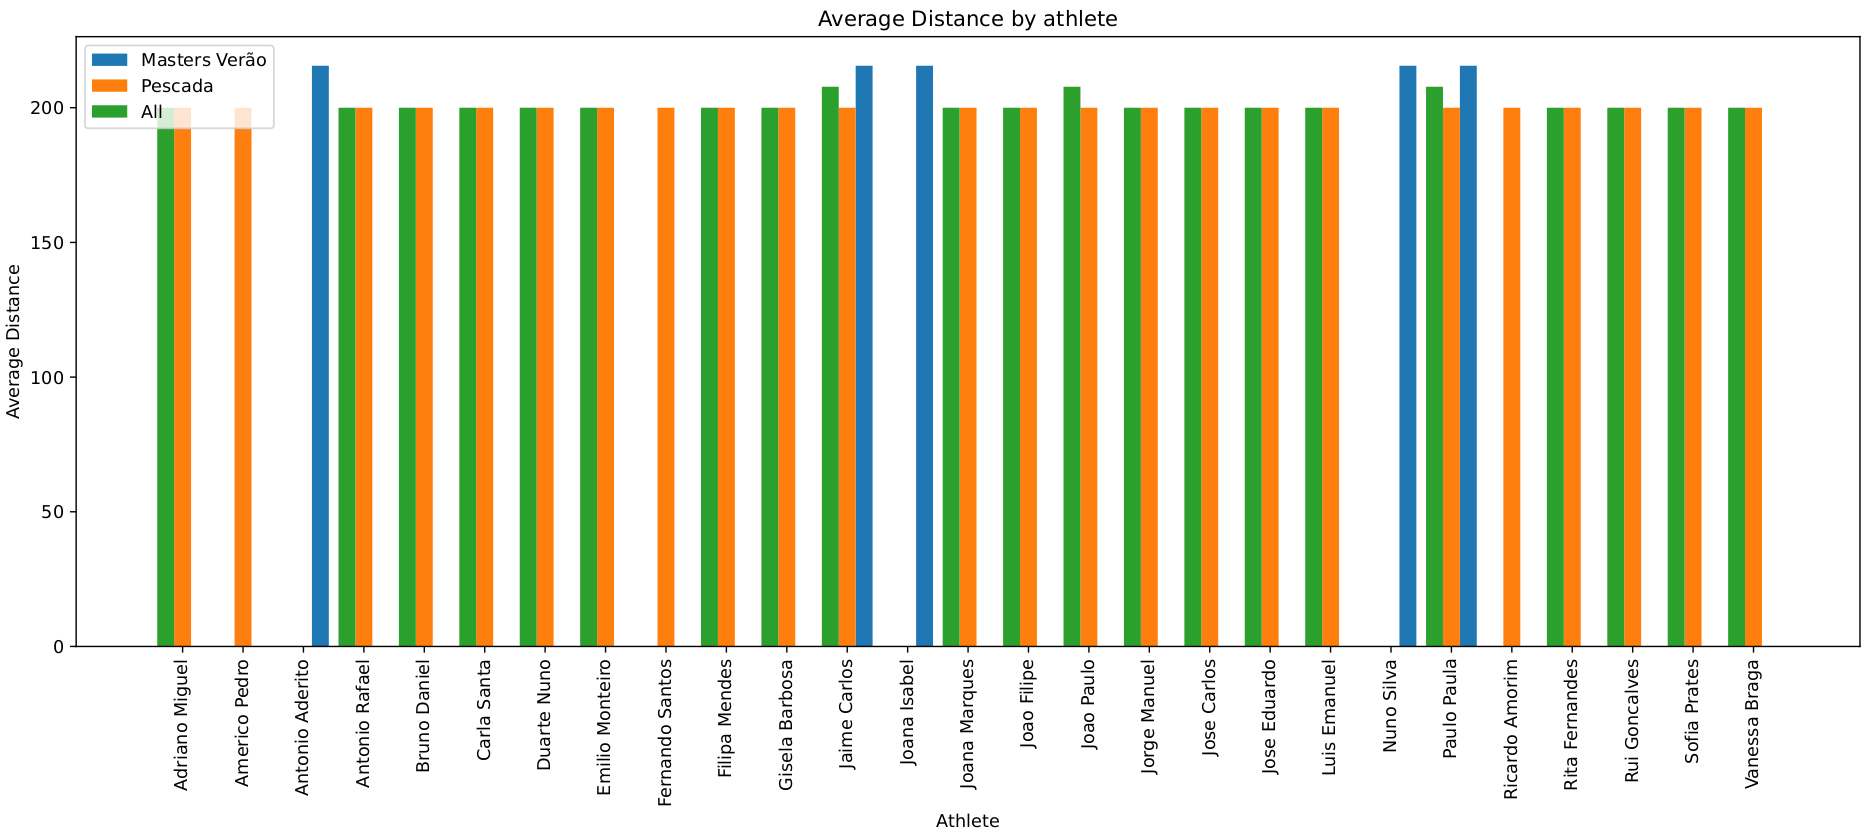
\includegraphics[width=\textwidth]{img/stats/ath1.png}
\end{figure}

\begin{figure}
    \centering
    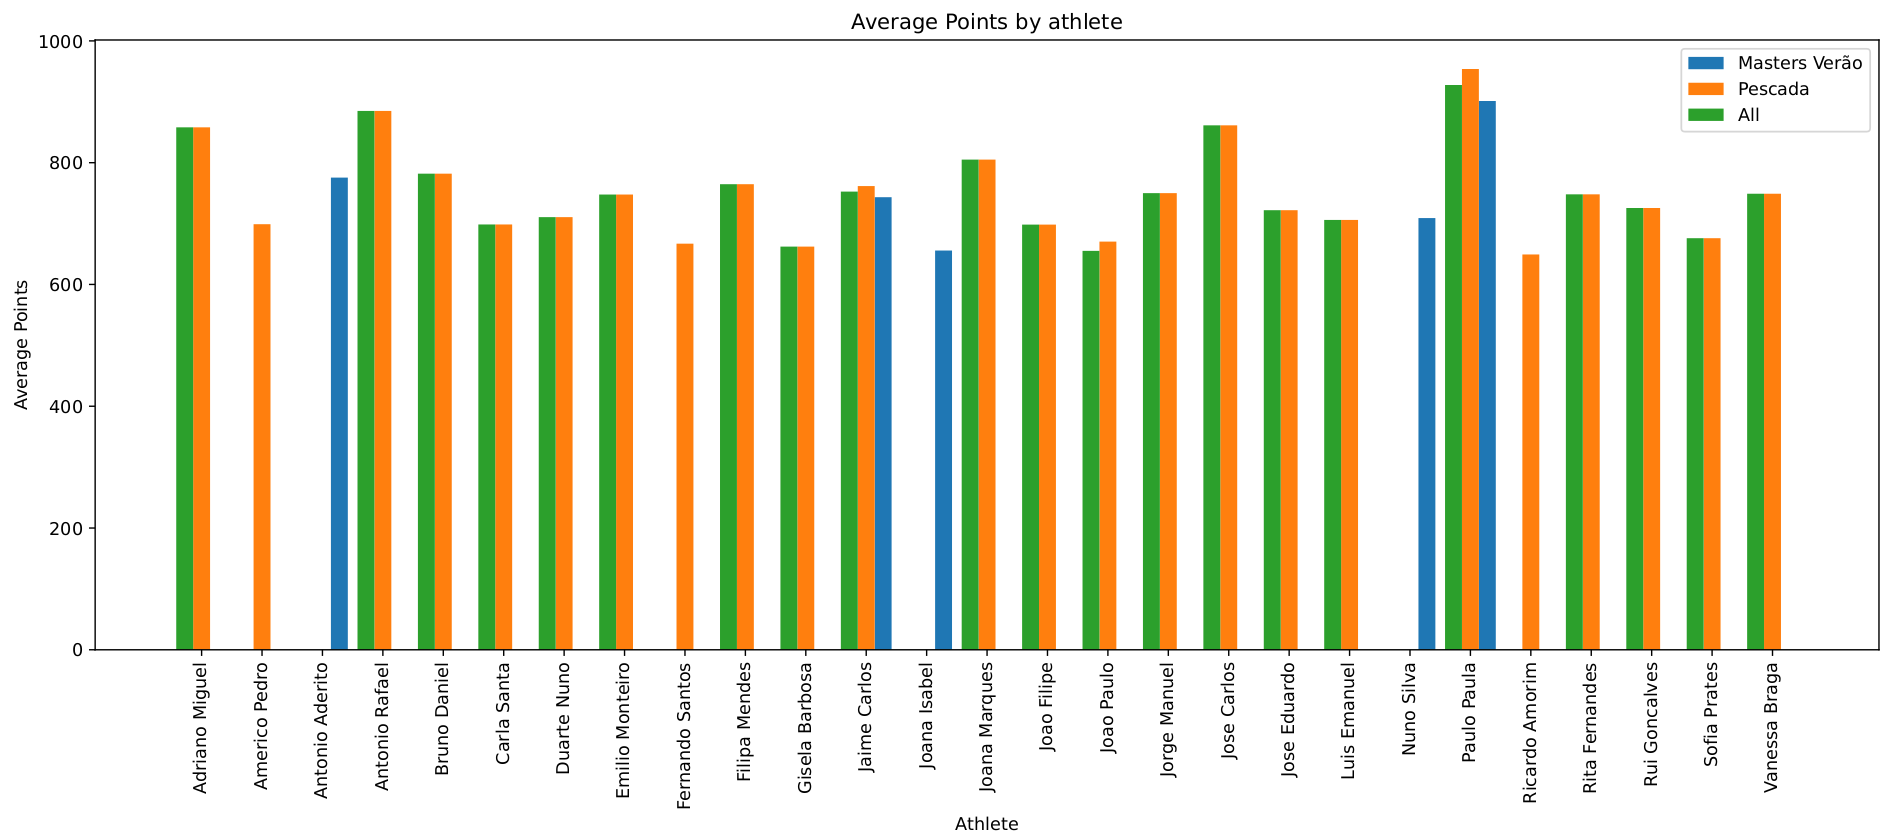
\includegraphics[width=\textwidth]{img/stats/ath2.png}
\end{figure}

\begin{figure}
    \centering
    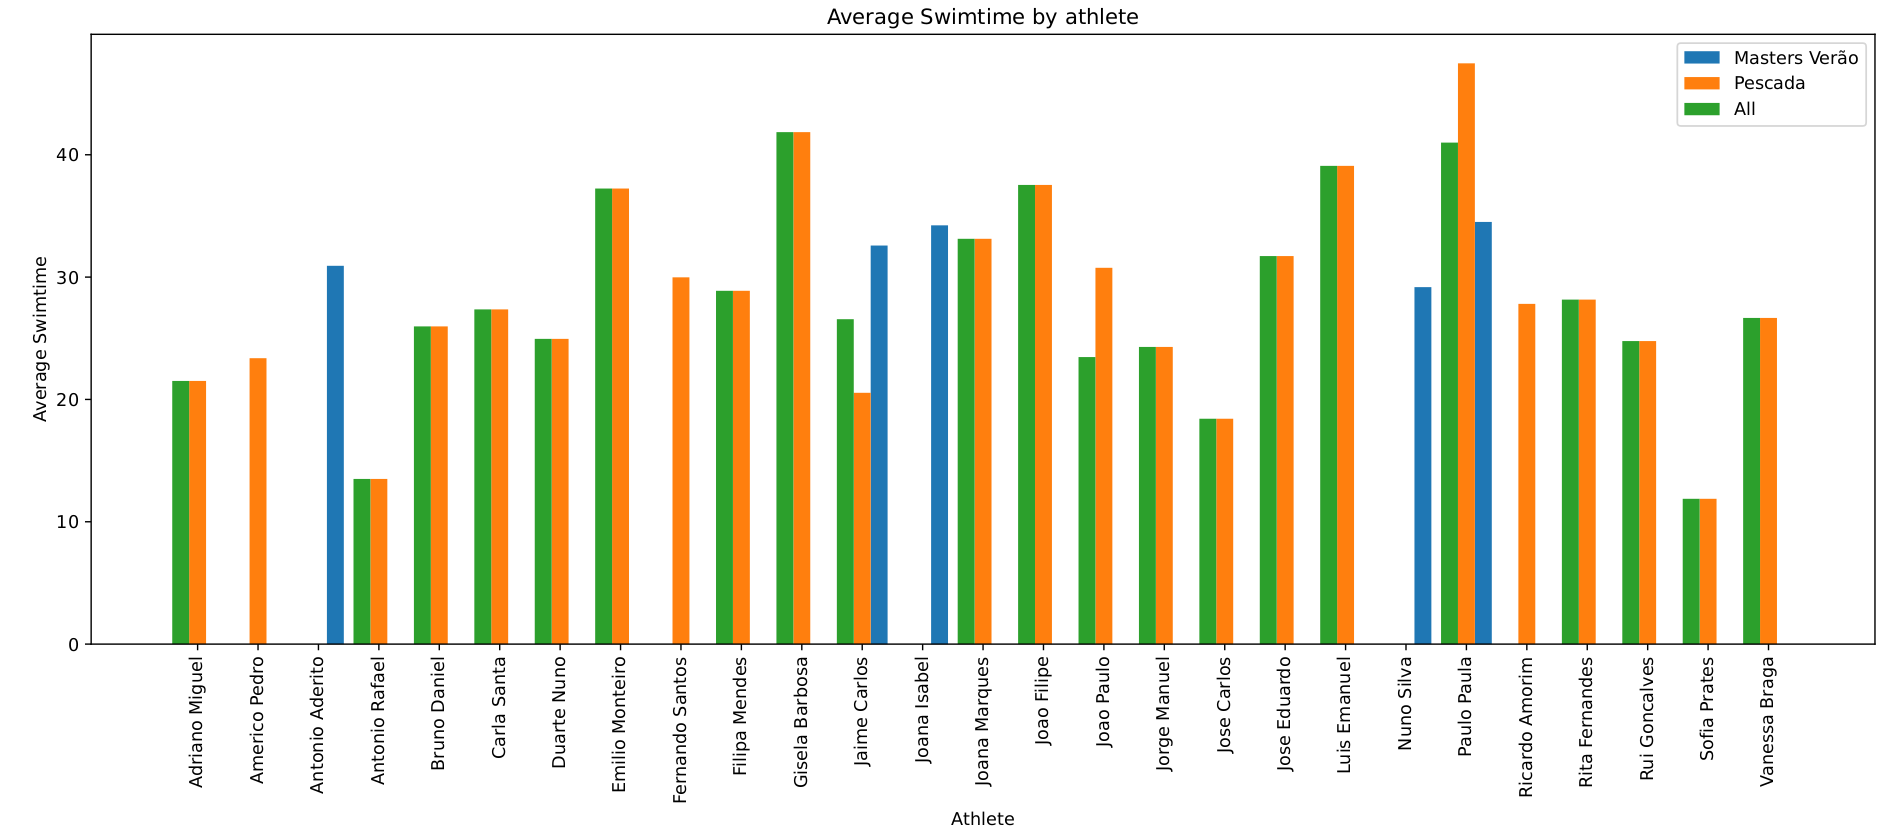
\includegraphics[width=\textwidth]{img/stats/ath3.png}
\end{figure}
\end{frame}

\end{document}
